%%\documentclass[a4paper,12pt,oneside]{llncs}
\documentclass{book}
%\usepackage[right=2cm,left=3cm,top=2cm,bottom=2cm,headsep=0cm]{geometry}

%%%%%%%%%%%%%%%%%%%%%%%%%%%%%%%%%%%%%%%%%%%%%%%%%%%%%%%%%%%
%% Juego de caracteres usado en el archivo fuente: UTF-8
\usepackage{ucs}
\usepackage[utf8x]{inputenc}
\usepackage{eurosym}

%%%%%%%%%%%%%%%%%%%%%%%%%%%%%%%%%%%%%%%%%%%%%%%%%%%%%%%%%%%
%% Juego de caracteres usado en la salida dvi
%% Otra posibilidad: \usepackage{t1enc}
\usepackage[T1]{fontenc}

%%%%%%%%%%%%%%%%%%%%%%%%%%%%%%%%%%%%%%%%%%%%%%%%%%%%%%%%%%%
%% Ajusta maergenes para a4
\usepackage{a4wide}

%%%%%%%%%%%%%%%%%%%%%%%%%%%%%%%%%%%%%%%%%%%%%%%%%%%%%%%%%%%
%% Uso fuente postscript times, para que los ps y pdf queden y pequeños...
\usepackage{times}

%%%%%%%%%%%%%%%%%%%%%%%%%%%%%%%%%%%%%%%%%%%%%%%%%%%%%%%%%%%
%% Posibilidad de hipertexto (especialmente en pdf)
\usepackage{hyperref}

%%%%%%%%%%%%%%%%%%%%%%%%%%%%%%%%%%%%%%%%%%%%%%%%%%%%%%%%%%%
%% Graficos 
\usepackage{graphics,graphicx}

%%%%%%%%%%%%%%%%%%%%%%%%%%%%%%%%%%%%%%%%%%%%%%%%%%%%%%%%%%%
%% Ciertos caracteres "raros"...
\usepackage{latexsym}

%%%%%%%%%%%%%%%%%%%%%%%%%%%%%%%%%%%%%%%%%%%%%%%%%%%%%%%%%%%
%% Matematicas aun más fuertes (american math dociety)
\usepackage{amsmath}

%%%%%%%%%%%%%%%%%%%%%%%%%%%%%%%%%%%%%%%%%%%%%%%%%%%%%%%%%%%
\usepackage{multirow} % para las tablas
\usepackage[spanish,es-tabla]{babel}

%%%%%%%%%%%%%%%%%%%%%%%%%%%%%%%%%%%%%%%%%%%%%%%%%%%%%%%%%%%
%% Fuentes matematicas lo mas compatibles posibles con postscript (times)
%% (Esto no funciona para todos los simbolos pero reduce mucho el tamaño del
%% pdf si hay muchas matamaticas....
\usepackage{mathptm}

%%% VARIOS:
%\usepackage{slashbox}
\usepackage{verbatim}
\usepackage{array}
\usepackage{listings}
\usepackage{multirow}
\usepackage{hhline}
\usepackage{titling}

%% MARCA DE AGUA
%% Este package de "draft copy" NO funciona con pdflatex
%%\usepackage{draftcopy}
%% Este package de "draft copy" SI funciona con pdflatex
%%%\usepackage{pdfdraftcopy}
%%%%%%%%%%%%%%%%%%%%%%%%%%%%%%%%%%%%%%%%%%%%%%%%%%%%%%%%%%%
%% Indenteacion en español...
\usepackage[spanish]{babel}
\usepackage{Estilos/Apuntes}
\usepackage[svgnames,x11names,table]{xcolor}
\usepackage{listingsutf8}
% Para escribir código en C
% \begin{verbatim}[language=C]
% #include <stdio.h>
% int main(int argc, char* argv[]) {
% puts("Hola mundo!");
% }
% \end{verbatim}
%\usepackage{hyphenat}
%
%\newenvironment{changemargin}[2]{%
%	\begin{list}{}{%
%			\setlength{\topsep}{0pt}%
%			\setlength{\leftmargin}{#1}%
%			\setlength{\rightmargin}{#2}%
%			\setlength{\listparindent}{\parindent}%
%			\setlength{\itemindent}{\parindent}%
%			\setlength{\parsep}{\parskip}%
%		}%
%		\item[]}{\end{list}}
%	
%\newenvironment{nota}{
%	\begin{changemargin}{2em}{2em}
%		\textbf{\textsc{Nota: }}
%	}{
%	\end{changemargin}
%}


\title{\huge{AWS vs Azure}}
\author{Jesús Rodríguez Heras\\
	Carlos Llamas Jaén\\
	Iván Castillo Caro\\
	Sisic Dino}


%%Configuracion del paquete listings
\lstset{language=bash, numbers=left, numberstyle=\tiny, numbersep=10pt, firstnumber=1, stepnumber=1, basicstyle=\small\ttfamily, tabsize=1, extendedchars=true, inputencoding=utf8/latin1, breaklines=true}

\begin{document}
	\maketitle
	
%	\thispagestyle{empty}
	\newpage{\pagestyle{empty}\cleardoublepage}
	
	\vspace*{\fill}
	La computación en la nube está a la orden del día, debido al abaratamieto de costes y la facilidad del escalado de los recursos empleados.
	
	Vamos a comparar las dos principales plataformas, Amazon Web Services y Microsoft Azure en términos centrados a la utilización de los recursos por dispositivos del Internet de las Cosas, muy relacionado con la computación en la nube.
	
	Primeramente comprobaremos como lanzar una máquina virtual en ambos servicios, útil para realizar los diversos cálculos que utiliza el sistema, posteriormente veremos como crear sitios o servicios web de cara a poder ser utilizados por los dispositivos para transmitir información y por último arrancaremos brokers de mensajería para la comunicación dispositivo-servidor.
	\vspace*{\fill}
	
	\tableofcontents
	\newpage
	
	\part{Introducción}
	\chapter{AWS}
\hypertarget{AWS}{}
\section{¿Qué es AWS?}
Amazon Web Services, en adelante AWS, es una colección de servicios de computación en la nube pública, también llamados servicios web\footnote{Es una tecnología que utiliza un conjunto de protocolos y estándares que sirven para intercambiar datos entre aplicaciones.}.

Es usado en aplicaciones como Dorpbox o Foursquare. Es una de las ofertas internacionales más importantes de la computación en la nube y compite directamente con \hyperlink{azure}{Microsoft Azure} aunque AWS es considerado como pionero en este campo.

\section{Historia}
AWS se lanza oficialmente en 2006 ofreciendo servicios en línea para otros sitios web o aplicaciones del lado del cliente.

La mayoría de estos servicios no están expuestos directamente a usuarios finales, sino que ofrecen una funcionalidad que otros desarrolladores puedan utilizar en sus aplicaciones.

El primer servicio de AWS lanzado para el uso público era Simple Queue Service (SQS). El cual es un servicio de colas de mensajes completamente administrado que permite desacoplar y ajustar la escala de microservicios, sistemas distribuidos y aplicaciones sin servidor. SQS elimina la complejidad y los gastos generales asociados con la gestión y el funcionamiento de middleware\footnote{Software que conecta componentes de software o aplicaciones para que puedan intercambiar datos entre ellas. Muy utilizado para soportar aplicaciones distribuidas.} orientado a mensajes, y permite a los desarrolladores centrarse en la diferenciación del trabajo.

Hoy en día, AWS proporciona una plataforma de infraestructura escalable, de confianza y de bajo costo en la nube que impula cientos de miles de negocios de 190 países de todo el mundo. Con centros de datos en Estados Unidos, Europa, Brasil, Singapur, Japón y Australia.

\section{Descripción}
Como ya se ha comentado anteriormente, AWS es una plataforma ideal para lanzar aplicaciones y proyectos de forma distribuida y escalable. Entre sus beneficios principales, podemos destacar las siguientes:
\begin{itemize}
	\item \textbf{Bajo costo:} AWS ofrece precios bajos por uso, sin gastos anticipados ni compromisos a largo plazo.
	\item \textbf{Agilidad y elasticidad instantánea:} AWS proporciona una infraestructura global y masiva en la nube que permite experimentar e iterar con rapidez. Puede implementar nuevas aplicaciones y aumentar su escala en cuanto crezca su carga de trabajo, oi bien, reducirla en función de la demanda.
	\item \textbf{Accesibilidad y flexibilidad:} AWS es una plataforma independiente del lenguaje y del sistema operativo.
	\item \textbf{Seguridad:} AWS es una plataforma tecnológica, segura y duradera que cuenta con certificaciones y auditorías reconocidas en el sector.
\end{itemize}
	\chapter{Azure}
En este capítulo se desarrollará la introducción de AWS.
	
	\part{Características y limitaciones}
	\chapter{AWS}
\section{Características}


\section{Limitaciones}


	\chapter{Características y limitaciones de Azure}
\section{Características}
Las características o servicios ofrecidos por Azure son los siguientes:
\begin{figure}[h]
	\centering
	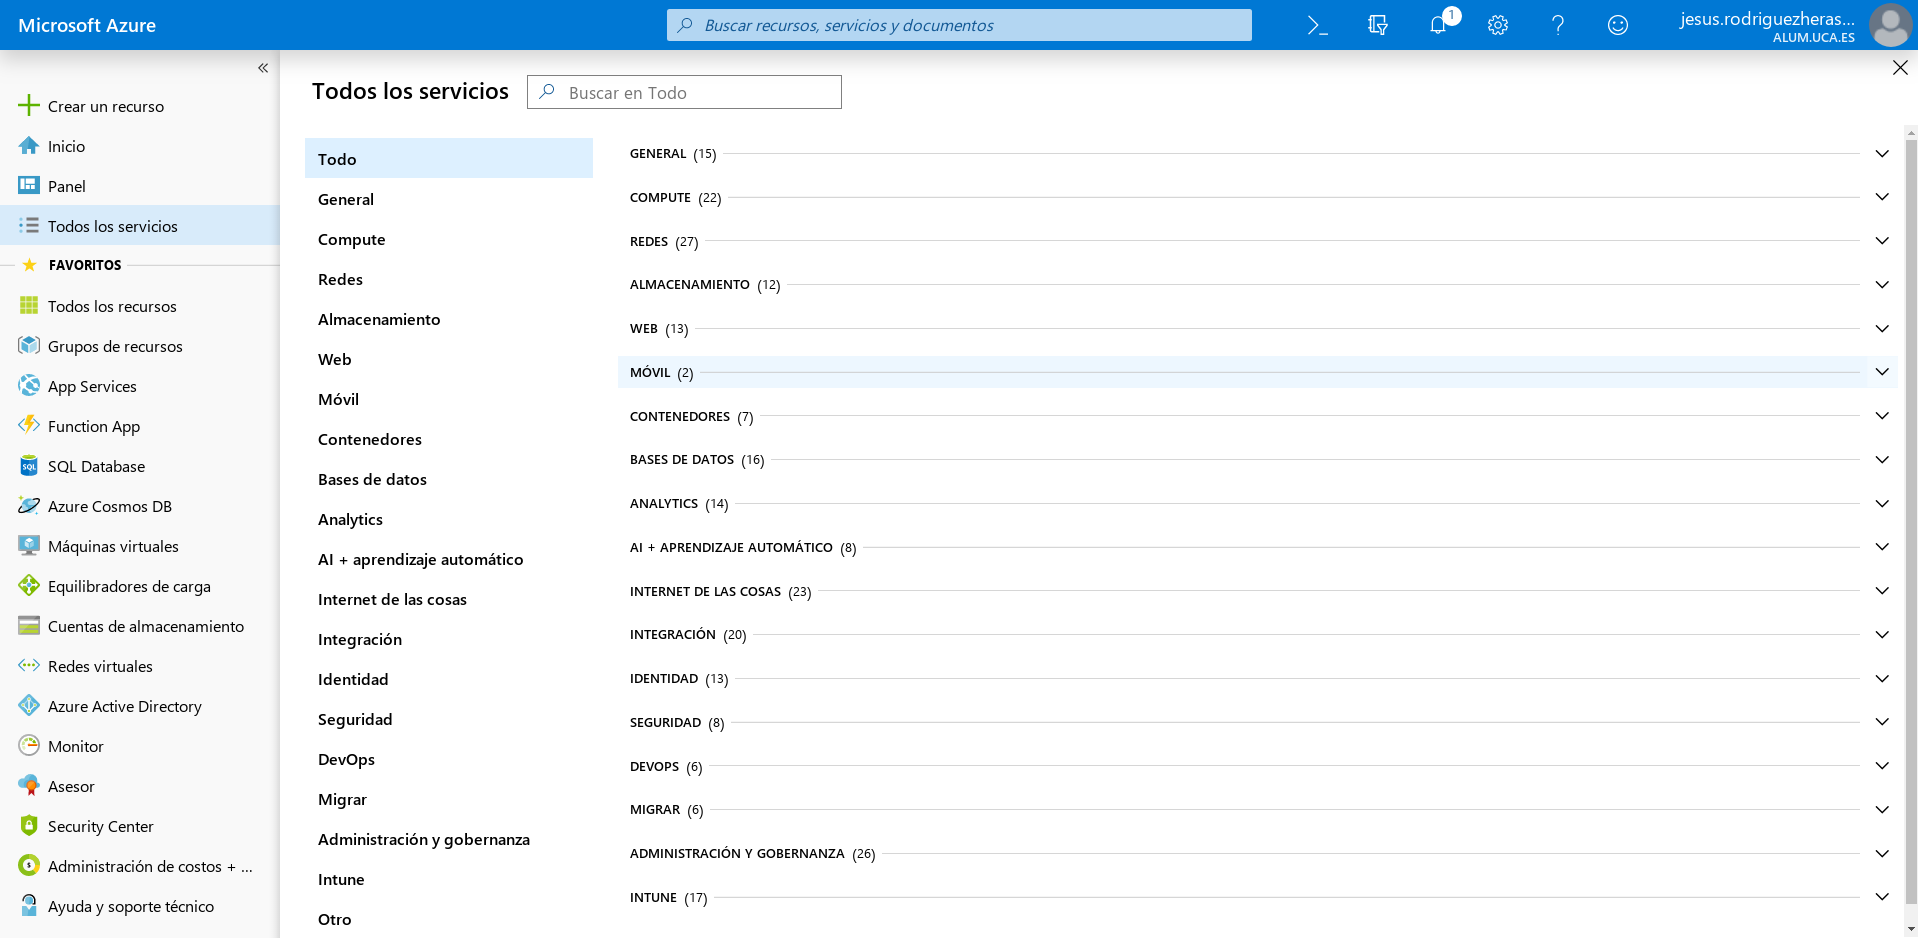
\includegraphics[scale=0.26]{ImagenesAzure/Servicios.png}
	\caption{Servicios ofrecidos por Azure.}
	\label{Servicios ofrecidos por Azure}
\end{figure}

Las características generales de Azure son las siguientes:
\begin{itemize}
	\item \textbf{Autoservicio bajo demanda:} Los usuarios pueden proveerse de cómputo en la nube sin requerir interacción humana o con el mismo proveedor.
	\item \textbf{Acceso ubicuo a la red:} Todo lo qeu podamos necesitar se encuentra en la red y accesible desde la red. Disponible desde cualquier dispositivo por medio de estándares como HTML o el protocolo HTTP.
	\item \textbf{Agrupación de recursos independientemente de la posición geográfica:} Los recursos del proveedor se encuentran geográficamente agrupados para servir a múltiples consumidores de manera distribuida y bajo demanda.
	\item \textbf{Elasticidad rápida:} Las funcionalidades se proporcionan de manera muy rápida, incluso puede ser configurable para que crezca dependiendo del ambiente actual.
	\item \textbf{Servicio medido:} El uso de todos los recursos se puede monitorizar, lo que proporciona transparencia tanto al que expone los servicios (el proveedor) como a los que acceden a ellos (los consumidores).
	\item \textbf{Pago por uso:} El costo de los servicios expuestos se puede modelar con la siguiente expresión:
	\begin{center}
		$(CaracterísticasDelServicio) * (TiempoDeActividad) = CostoTotal$
	\end{center}
\end{itemize}

Cabe destacar, y, como se ve en la figura \ref{Servicios ofrecidos por Azure} que en Azure sí contamos con servicios relacionados con Inteligencia Artificial y aprendizaje automático (Machine Learning).

\section{Limitaciones}
Dentro de la capa de estudiantes\footnote{La que hemos podido probar gracias al acuerdo de la UCA con Microsoft.} tenemos las siguientes \href{https://azure.microsoft.com/es-es/free/free-account-students-faq/}{limitaciones}, de las cuales, las más destacables son (entre muchas otras):
\begin{itemize}
	\item 750 horas de máquinas virtuales B1S\footnote{Características de las máquinas B1S: 1vCPU, 1GiB de RAM y 4GiB de almacenamiento.} tanto para Linux como para Windows.
	\item 128GB de Managed Disks\footnote{Ofrece la seguridad, disponibilidad, escalabilidad y durabilidad de HDD/SSD que se necesite para todas las cargas de trabajo, desde cargas de trabajo críticas hasta escenarios de prueba.} como combinación de dos discos de almacenamiento SSD de 64GB, además de 1GB en operaciones instantáneas y 2 millones de operaciones de E/S.
	\item 250GB de una instancia S0\footnote{Instancia de bases de datos gestionada por Azure SQL.} estándar de bases de datos SQL con 10 unidades de transacción de bases de datos.
	\item 1500 horas de IP dinámica para máquinas virtuales B1S.
\end{itemize}
	
	\part{Comparación de los servicios ofrecidos por AWS y Azure}
	\chapter{Creación de máquinas virtuales en AWS y Azure}
En este capítulo se describe la creación de máquinas virtuales en los servicios de AWS y Azure para ver la escalabilidad que proporcionan dichos servicios.

Hemos seleccionado las siguientes máquinas virtuales en función del servicio:
\begin{itemize}
	\item \textbf{AWS:} Hemos seleccionado una máquina EC2, la cual proporciona capacidad de computación escalable en la nube de AWS. El uso de Amazon EC2 elimina la necesidad de invertir inicialmente en hardware, de manera que puede desarrollar e implementar aplicaciones en menos tiempo. Puede usar Amazon EC2 para lanzar tantos servidores virtuales como necesite, configurar la seguridad y las redes y administrar el almacenamiento.
	\item \textbf{Azure:} Hemos seleccionado una máquina B1ls la cual es la opción ideal para servidores web pequeños, bases de datos pequeñas y entornos de desarrollo y pruebas. Ofrece una forma económica de implementar cargas de trabajo que no necesitan el uso pleno de la CPU de forma continuada e irrumpen en su rendimiento.
\end{itemize}
\section{Creación de una máquina virtual en AWS}
La máquina t2.micro de Amazon EC2 seleccionada cuenta con las siguientes especificaciones técnicas:
\begin{itemize}
	\item Un vCPU.
	\item 1 GB de RAM.
	\item 8 GB de almacenamiento (HDD o SSD).
\end{itemize}

Para crear el servicio debemos seguir los siguientes pasos:
\newpage
\begin{enumerate}
	\item Nos dirigimos a la consola de administración de AWS.
	\begin{figure}[h]
		\centering
		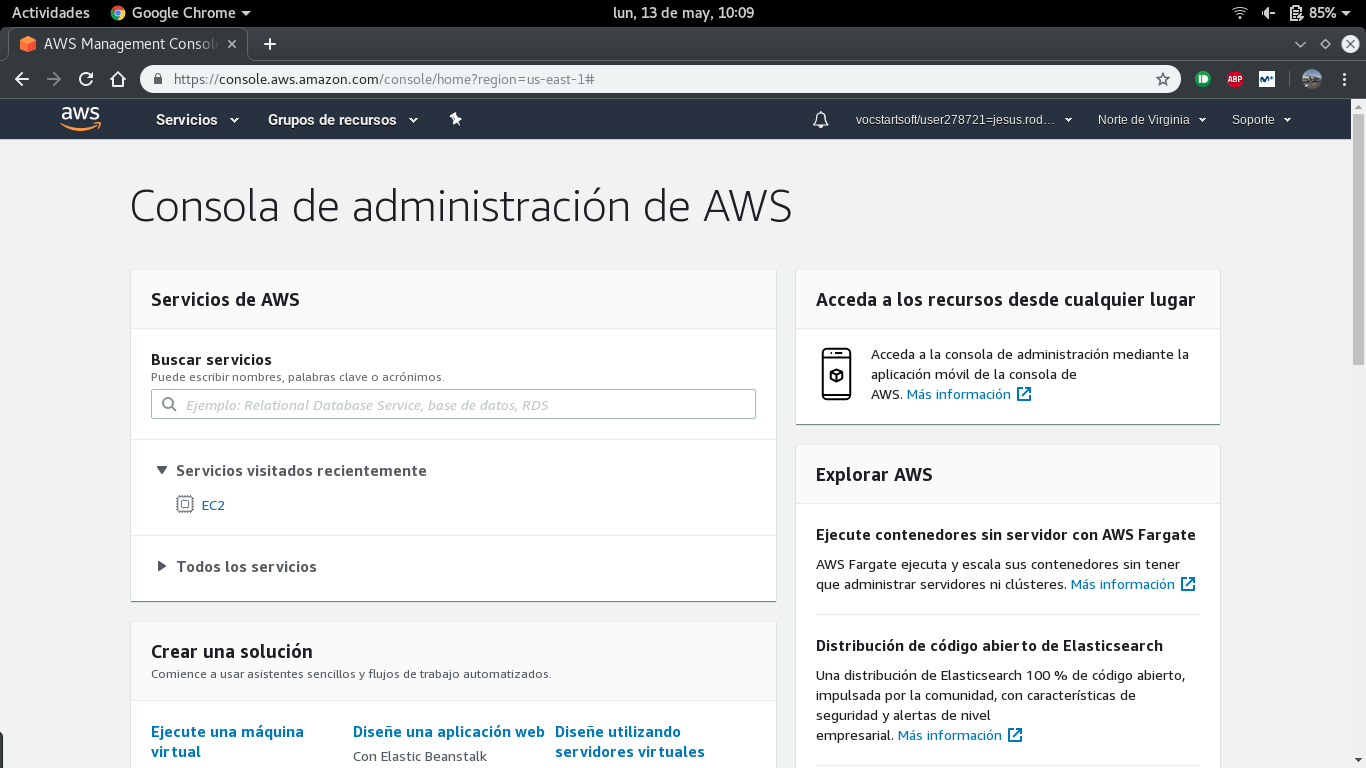
\includegraphics[scale=0.28]{ImagenesAWS/MV/1.png}
		\caption{Consola de administración de AWS.}
		\label{Consola de administración de AWS}
	\end{figure}
	\item Seleccionamos ``Ejecute una máquina virtual''.
	\begin{figure}[h]
		\centering
		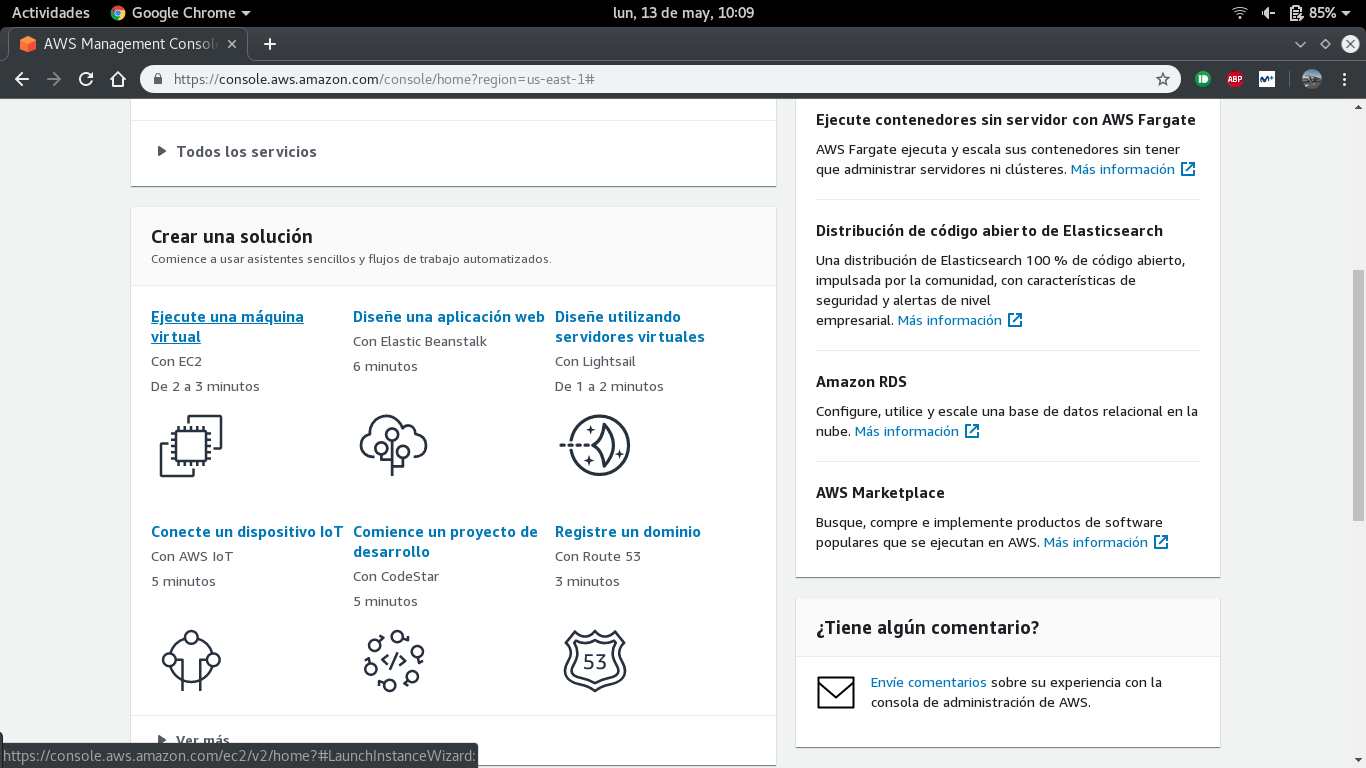
\includegraphics[scale=0.28]{ImagenesAWS/MV/3.png}
		\caption{Selección de solución.}
		\label{Selección de solución}
	\end{figure}
\newpage
	\item Seleccionamos la AMI que deseemos, en nuestro caso será ``Ubuntu server 18.04 LTS (HVM), SSD Volume Type''.
	\begin{figure}[h]
		\centering
		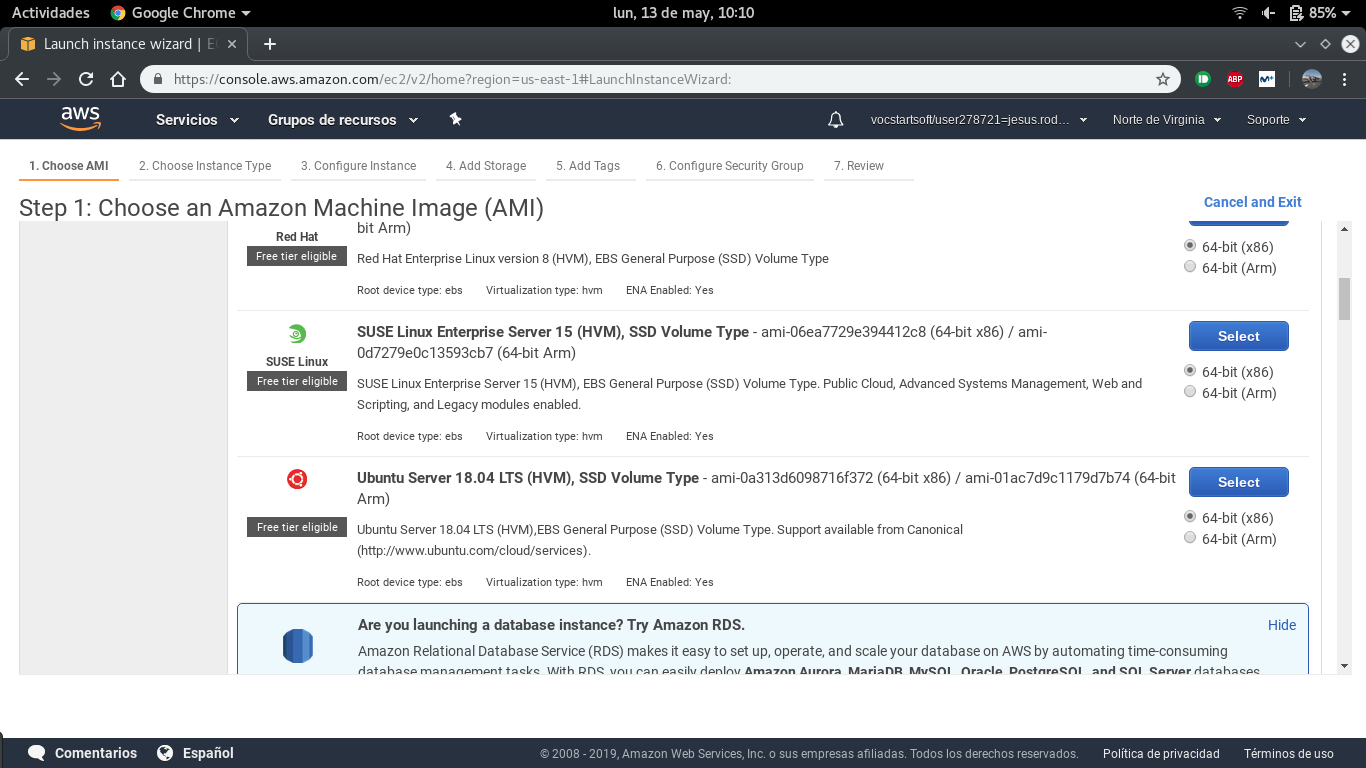
\includegraphics[scale=0.28]{ImagenesAWS/MV/5.png}
		\caption{Selección de AMI.}
		\label{Selección de AMI}
	\end{figure}
	\item Seleccionamos el tipo de instancia que queremos:
	\begin{figure}[h]
		\centering
		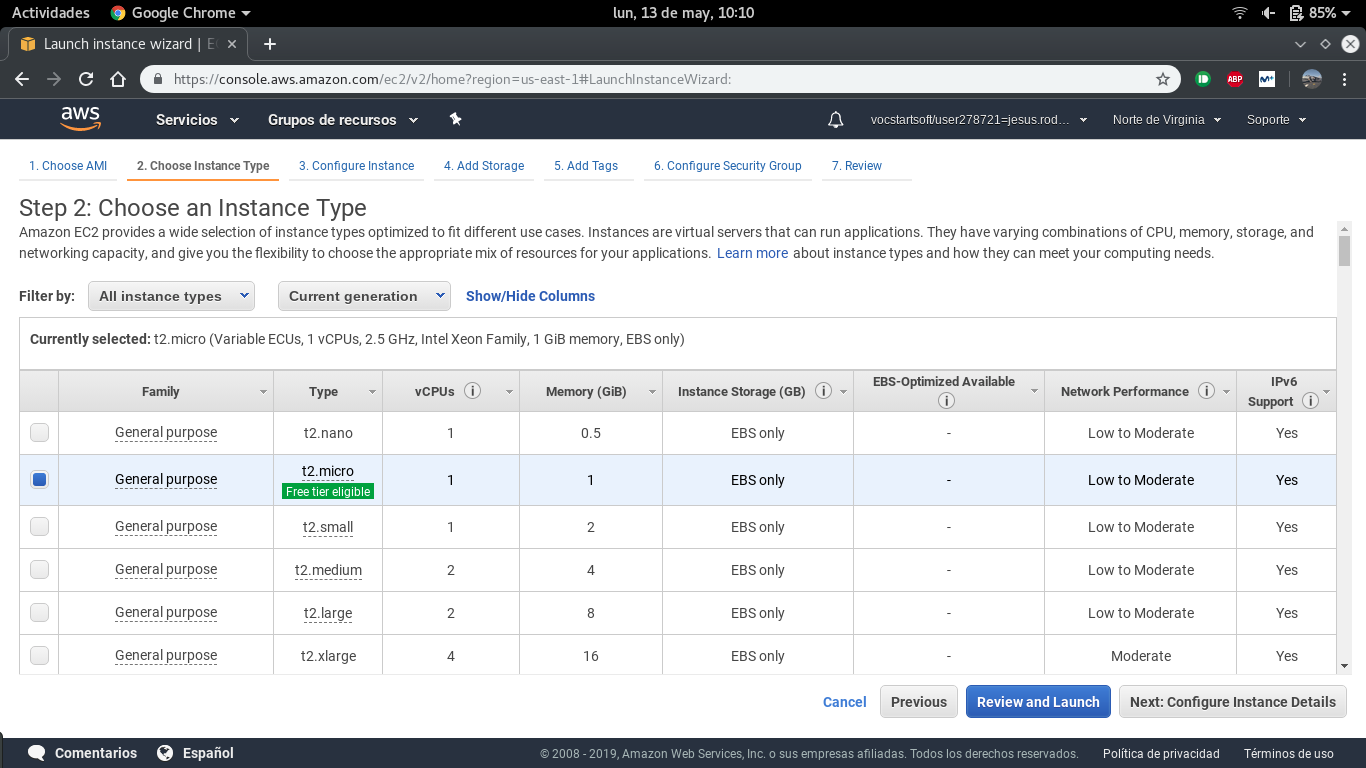
\includegraphics[scale=0.28]{ImagenesAWS/MV/6.png}
		\caption{Selección de instancia.}
		\label{Selección de instancia}
	\end{figure}
\newpage
	\item Ahora debemos configurar los detalles que tendrá la instancia seleccionada:
	\begin{figure}[h]
		\centering
		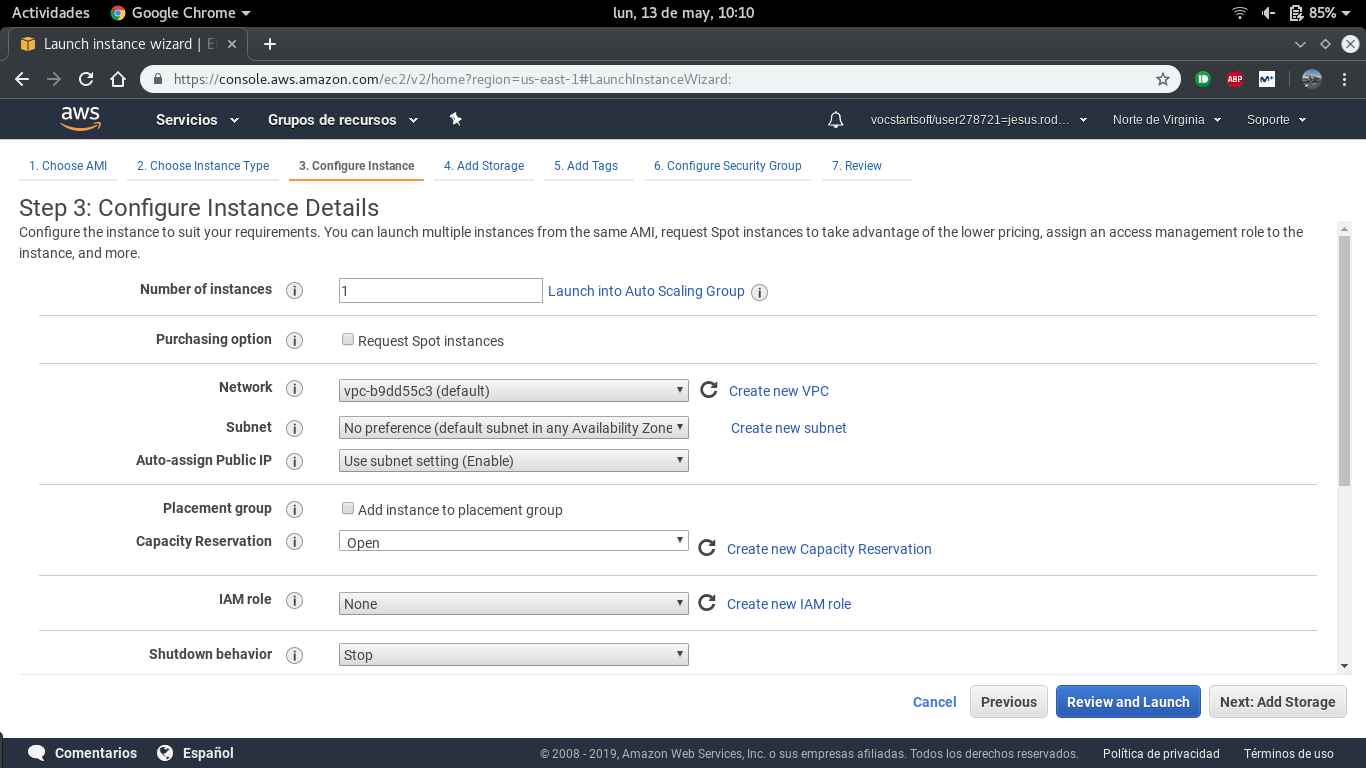
\includegraphics[scale=0.28]{ImagenesAWS/MV/7.png}
		\caption{Configuración de la instancia.}
		\label{Configuración de la instancia}
	\end{figure}
	\item Seleccionamos el tamaño del almacenamiento y el tipo de disco duro:
	\begin{figure}[h]
		\centering
		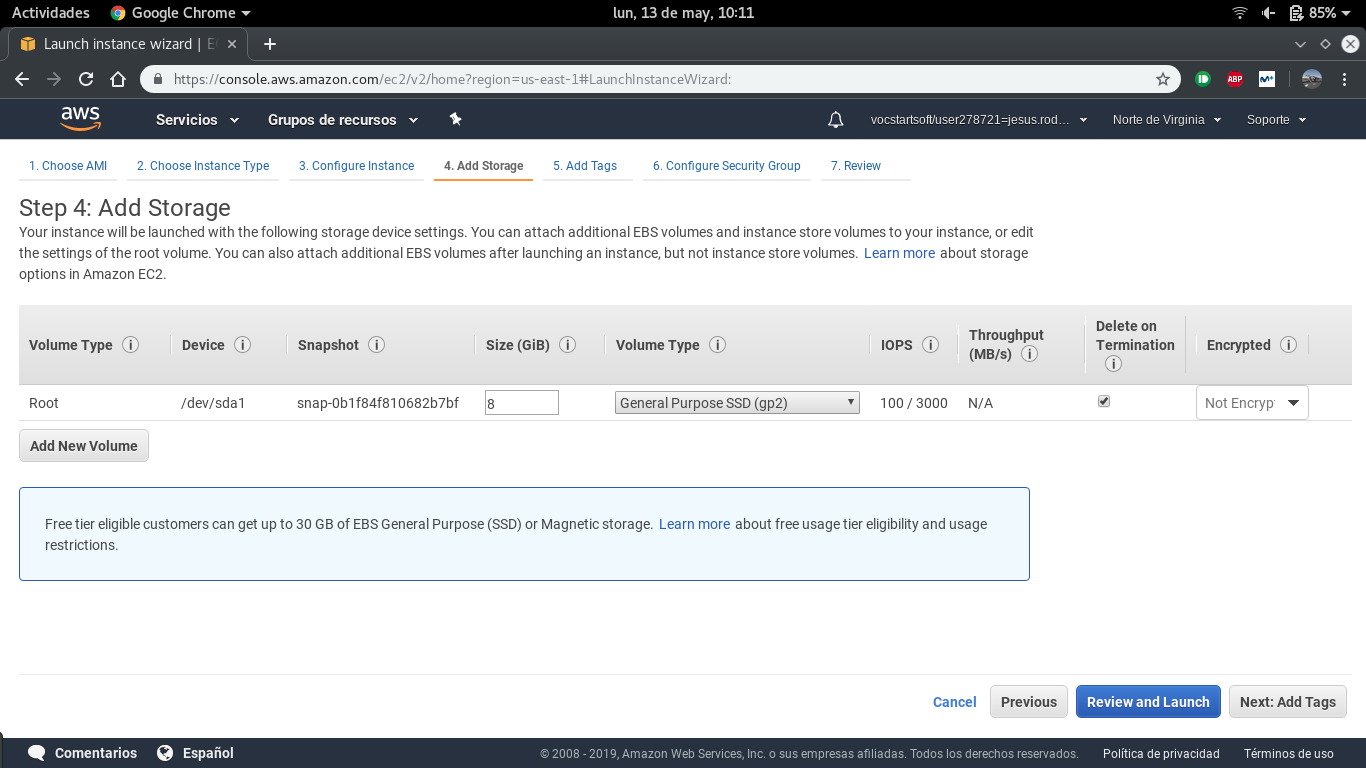
\includegraphics[scale=0.28]{ImagenesAWS/MV/8.png}
		\caption{Selección de almacenamiento.}
		\label{Selección de almacenamiento}
	\end{figure}
\newpage
	\item Añadimos las etiquetas que deseemos:
	\begin{figure}[h]
		\centering
		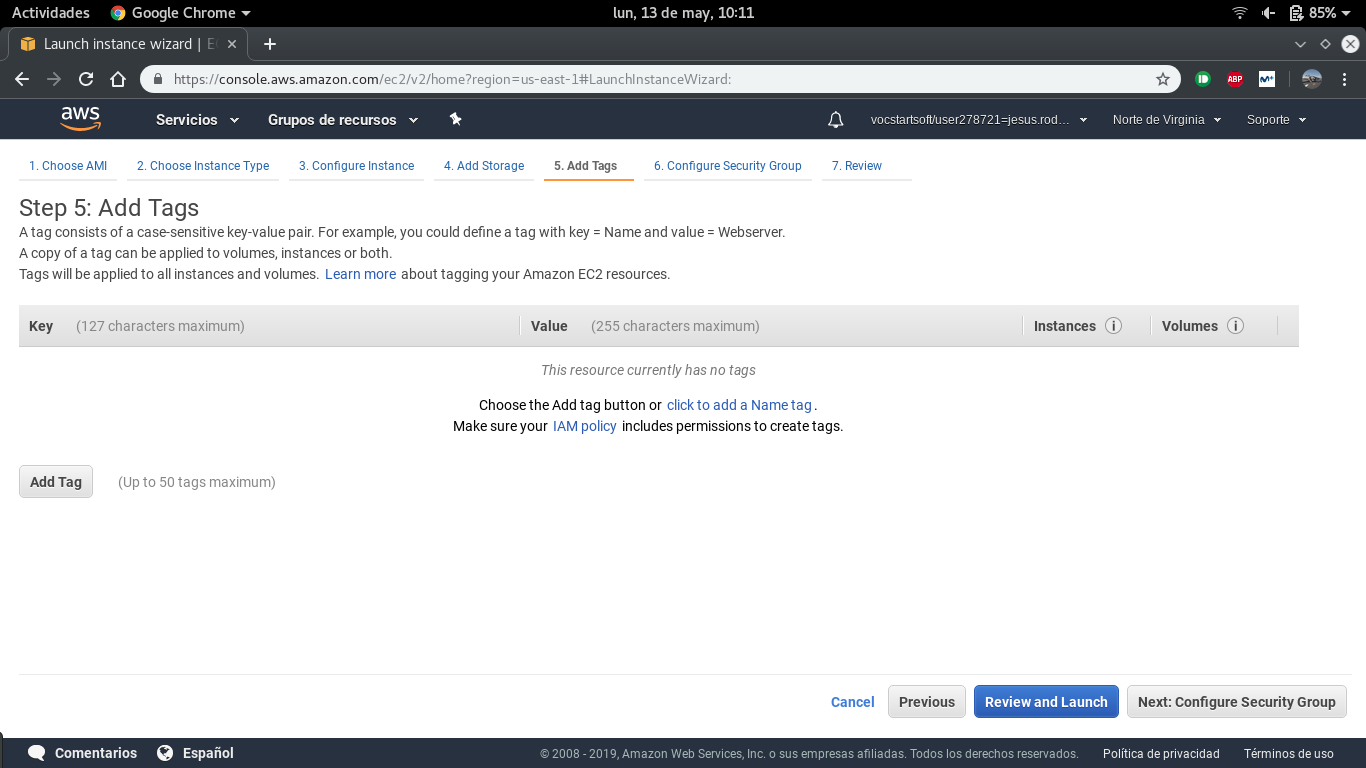
\includegraphics[scale=0.28]{ImagenesAWS/MV/9.png}
		\caption{Añadimos las etiquetas.}
		\label{Añadimos las etiqutas}
	\end{figure}
	\item Configuramos las conexiones que vayamos a tener como el SSH:
	\begin{figure}[h]
		\centering
		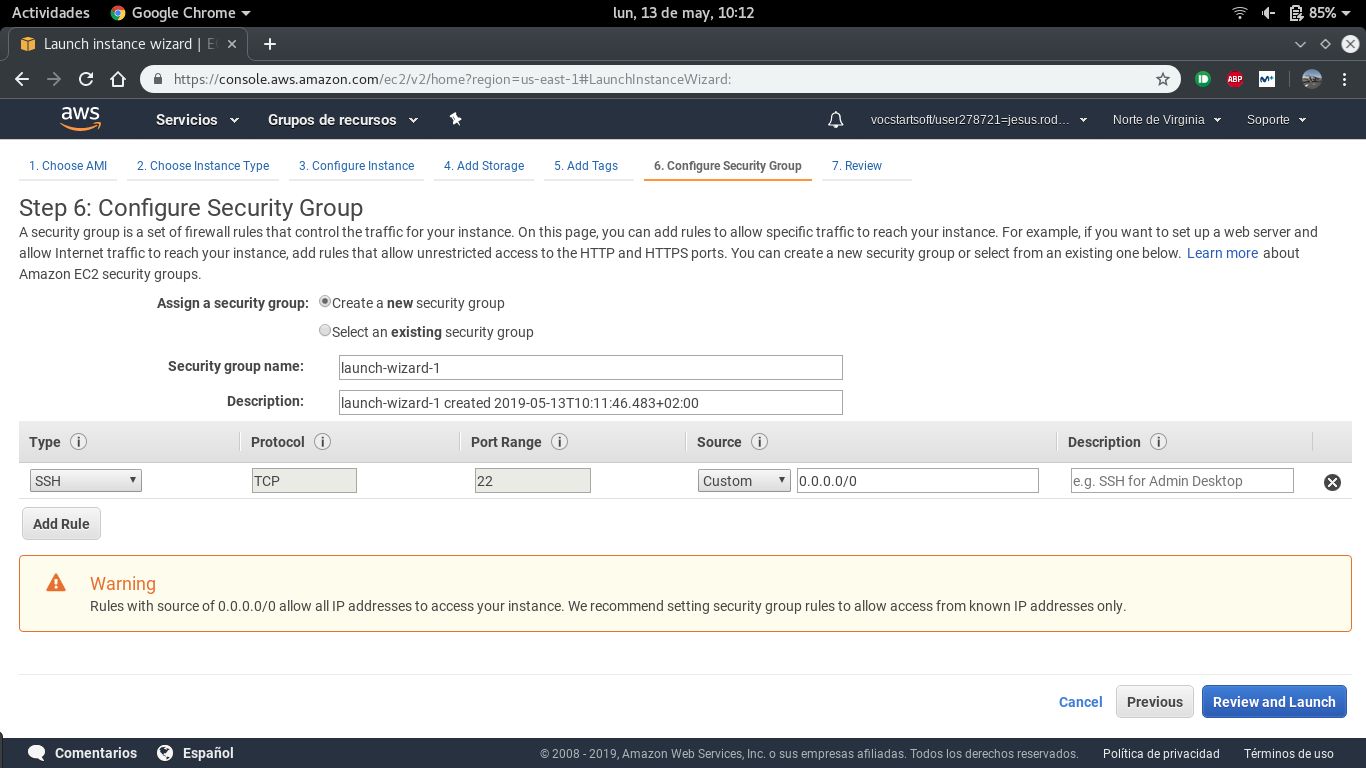
\includegraphics[scale=0.28]{ImagenesAWS/MV/10.png}
		\caption{Configuración conexiones.}
		\label{Configuración de conexiones}
	\end{figure}
\newpage
	\item Finalmente, veremos una página con el resumen de las características que tendrá nuestra máquina:
	\begin{figure}[h]
		\centering
		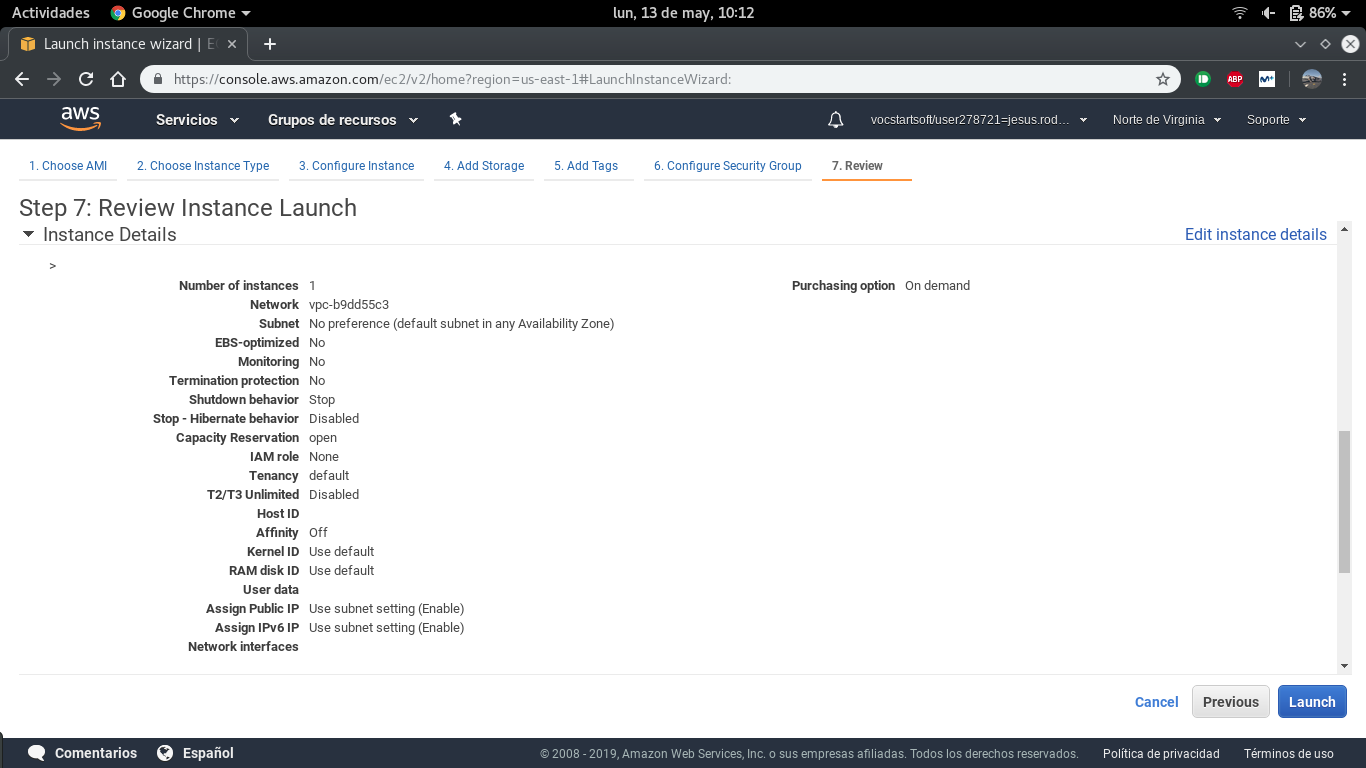
\includegraphics[scale=0.28]{ImagenesAWS/MV/12.png}
		\caption{Resumen de la máquina.}
		\label{Resumen de la máquina}
	\end{figure}
	\item Cuando le damos a ``Launch'' nos saldrá la siguiente pestaña para generar y descargar la clave SSH:
	\begin{figure}[h]
		\centering
		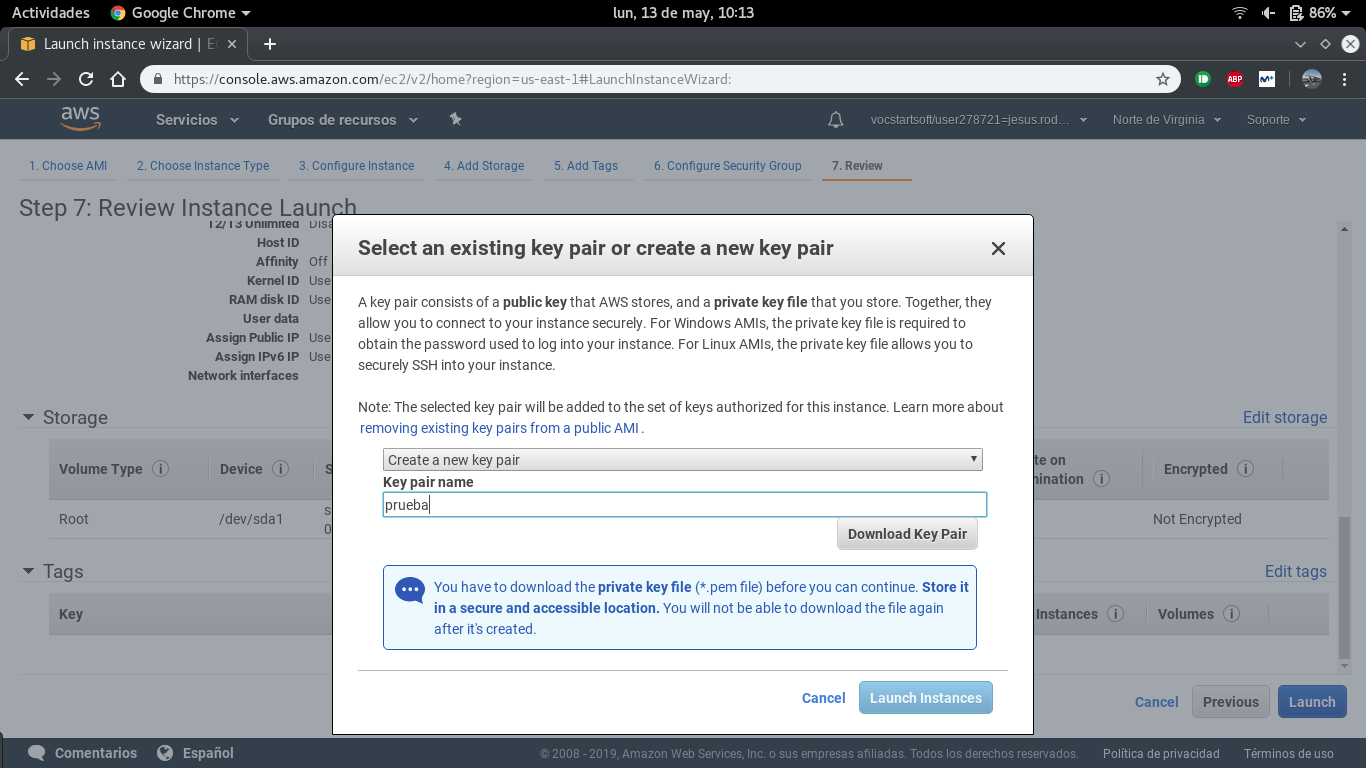
\includegraphics[scale=0.28]{ImagenesAWS/MV/13.png}
		\caption{Creación de clave SSH.}
		\label{Creación de clave SSH}
	\end{figure}
\newpage
	\item Luego, en el apartado de ``Instancias'' de la consola de administración podremos ver nuestra máquina virtual ejecutándose:
	\begin{figure}[h]
		\centering
		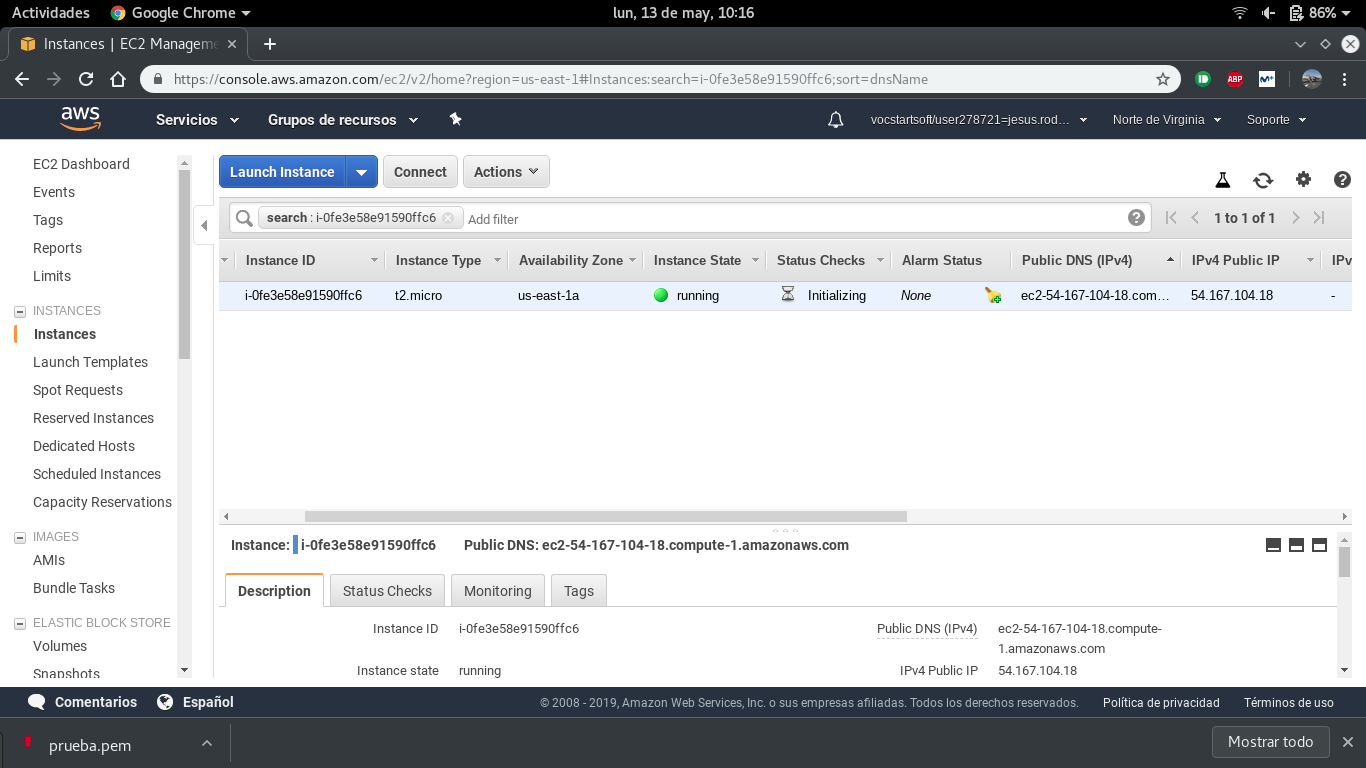
\includegraphics[scale=0.28]{ImagenesAWS/MV/15.png}
		\caption{Máquina en ejecución.}
		\label{Máquina en ejecución}
	\end{figure}
	\item Para conectarnos a la máquina por SSH, debemos cambiar los permisos del fichero ``prueba.pem'' generado e introducir el siguiente comando:
	\begin{center}
		\texttt{ssh -i prueba.pem ubuntu@54.167.104.18}
	\end{center}
	\begin{figure}[h]
		\centering
		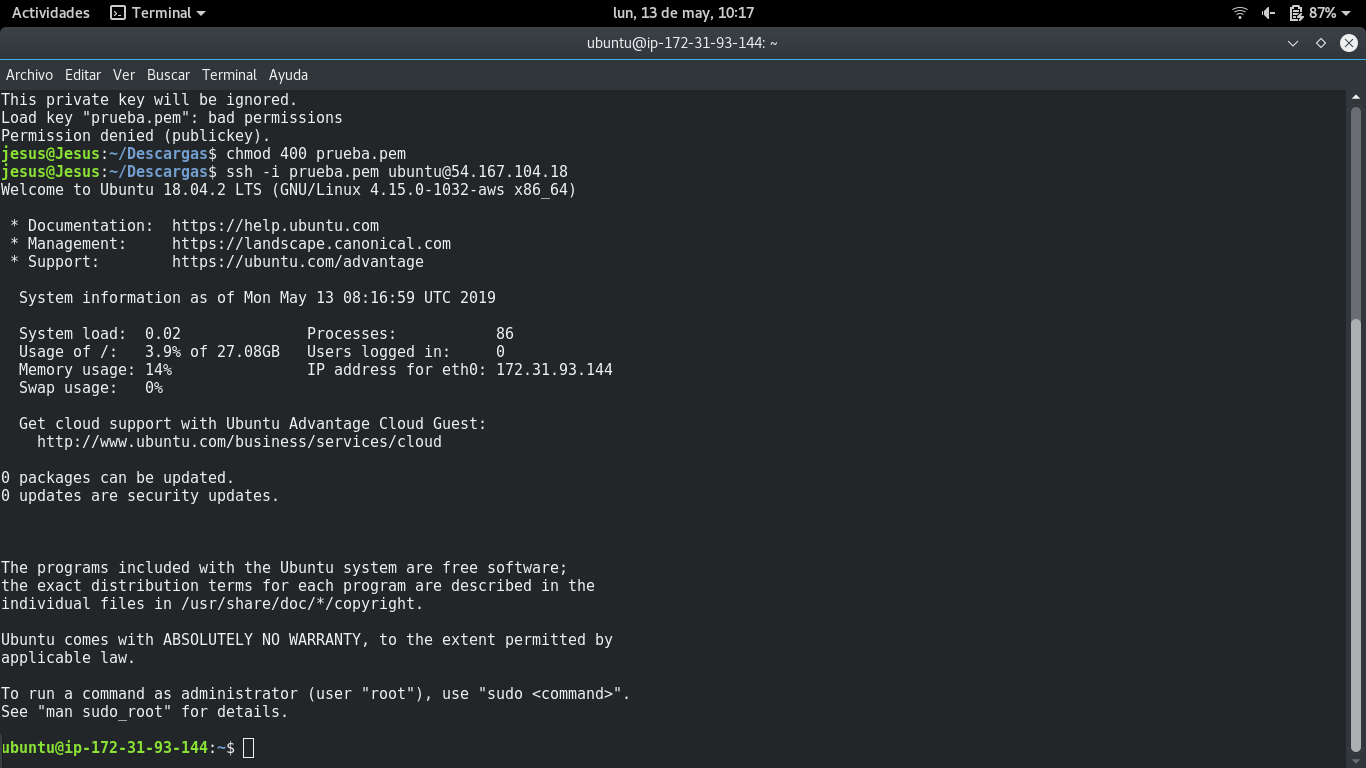
\includegraphics[scale=0.28]{ImagenesAWS/MV/16.png}
		\caption{Conexión con la máquina virtual.}
		\label{Conexión con la máquina virtual}
	\end{figure}
\newpage
	\item Si lanzamos el comando: \texttt{cat /proc/cpuinfo}, podremos ver las características del procesador de nuestra máquina virtual.
	\begin{figure}[h]
		\centering
		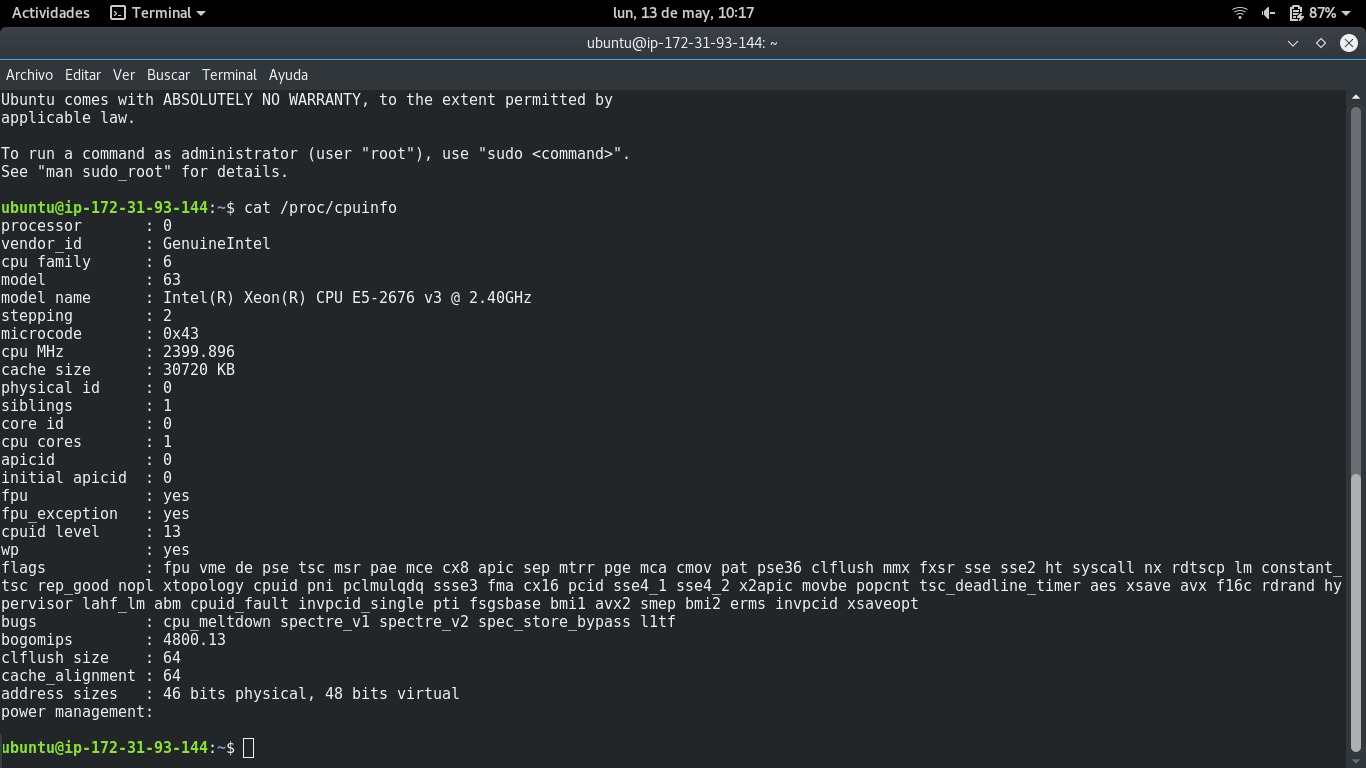
\includegraphics[scale=0.28]{ImagenesAWS/MV/17.png}
		\caption{Información de la CPU de la máquina virtual.}
		\label{Información de la CPU de la máquina virtual}
	\end{figure}
	\item Para detener la ejecución de la máquina virtual, en la consola de administración, hacemos click derecho y seleccionamos ``Stop'' dentro de ``Instance State''. También es posible detener la máquina virtual con el comando \texttt{sudo shutdown now}.
	\begin{figure}[h]
		\centering
		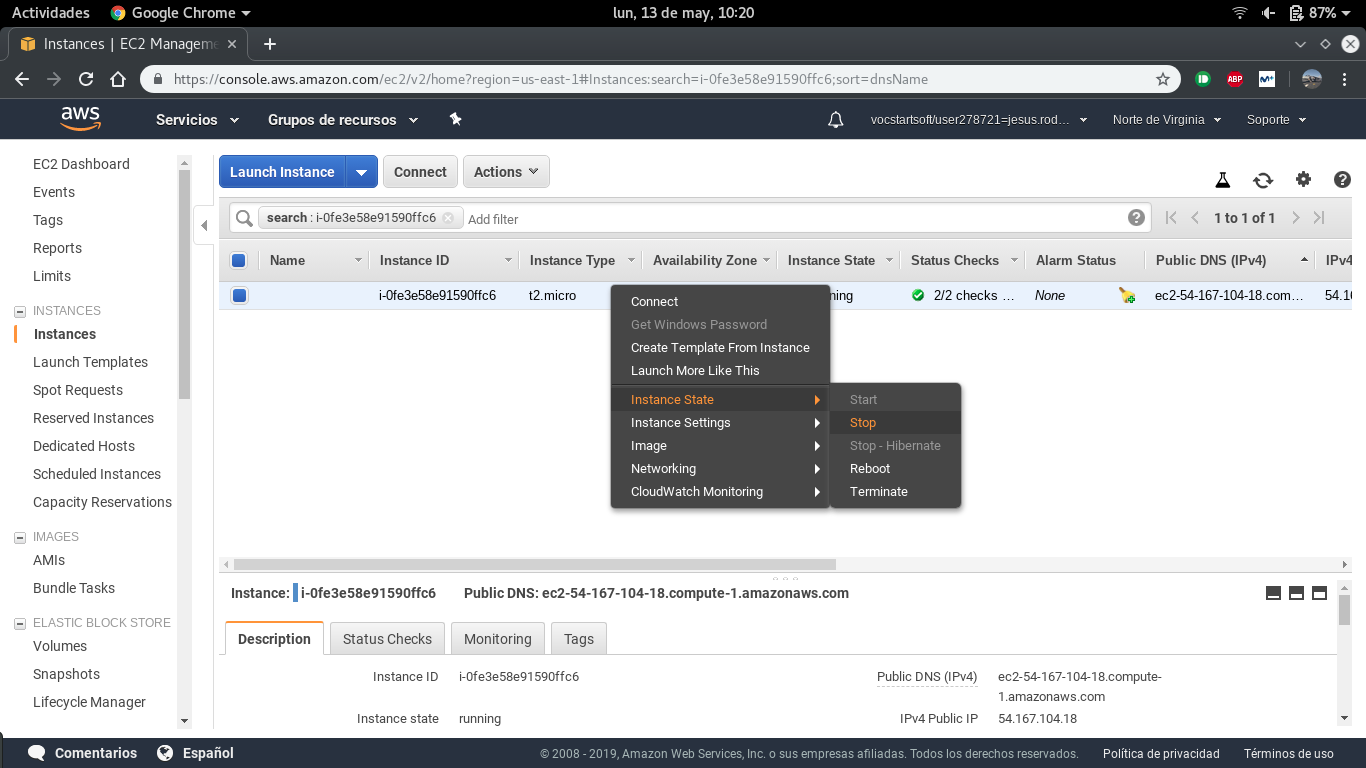
\includegraphics[scale=0.28]{ImagenesAWS/MV/19.png}
		\caption{Detener la ejecución de la máquina virtual.}
		\label{Detener la ejecución de la máquina virtual}
	\end{figure}
\end{enumerate}

\newpage
\section{Creación de una máquina virtual en Azure}
La máquina B1ls de Azure seleccionada cuenta con las siguientes especificaciones técnicas:
\begin{itemize}
	\item Un vCPU.
	\item 0.5 GB de RAM.
	\item 4 GB de almacenamiento (HDD o SSD).
	\item 200 MB de transferencia.
\end{itemize}

Para crear el servicio, debemos seguir los siguientes pasos:
\begin{enumerate}
	\item Seleccionamos la opción ``máquinas virtuales'' del menú de la derecha:
	\begin{figure}[h]
		\centering
		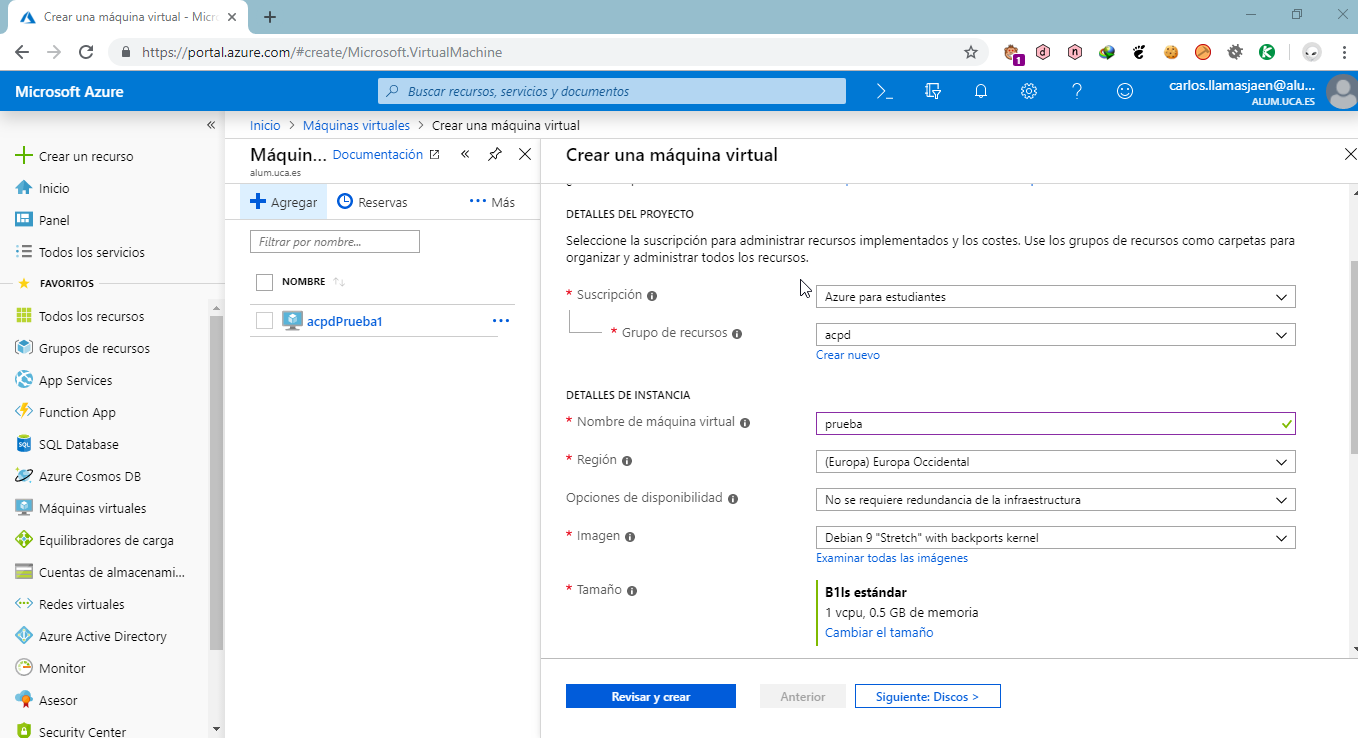
\includegraphics[scale=0.35]{ImagenesAzure/MV/1.png}
		\caption{Crear máquina virtual.}
		\label{Crear máquina virtual}
	\end{figure}
\newpage
	\item Seleccionamos el tipo de instancia que queremos:
	\begin{figure}[h]
		\centering
		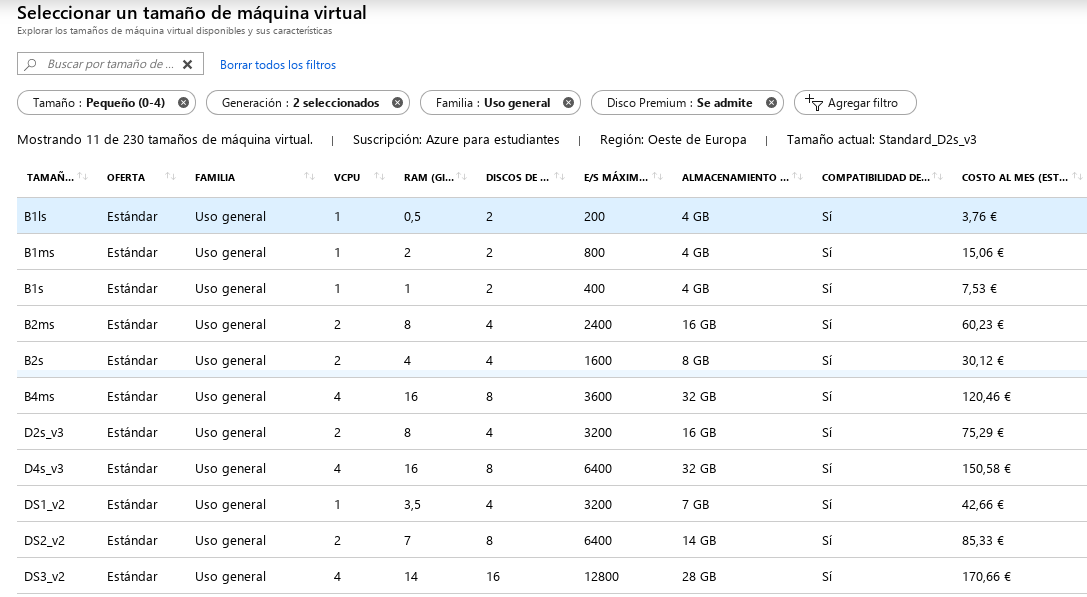
\includegraphics[scale=0.35]{ImagenesAzure/MV/1medio.png}
		\caption{Selección de instancia.}
		\label{Selección de instancia2}
	\end{figure}
	\item Establecemos el tipo de autenticación por SSH y añadimos la clave pública:
	\begin{figure}[h]
		\centering
		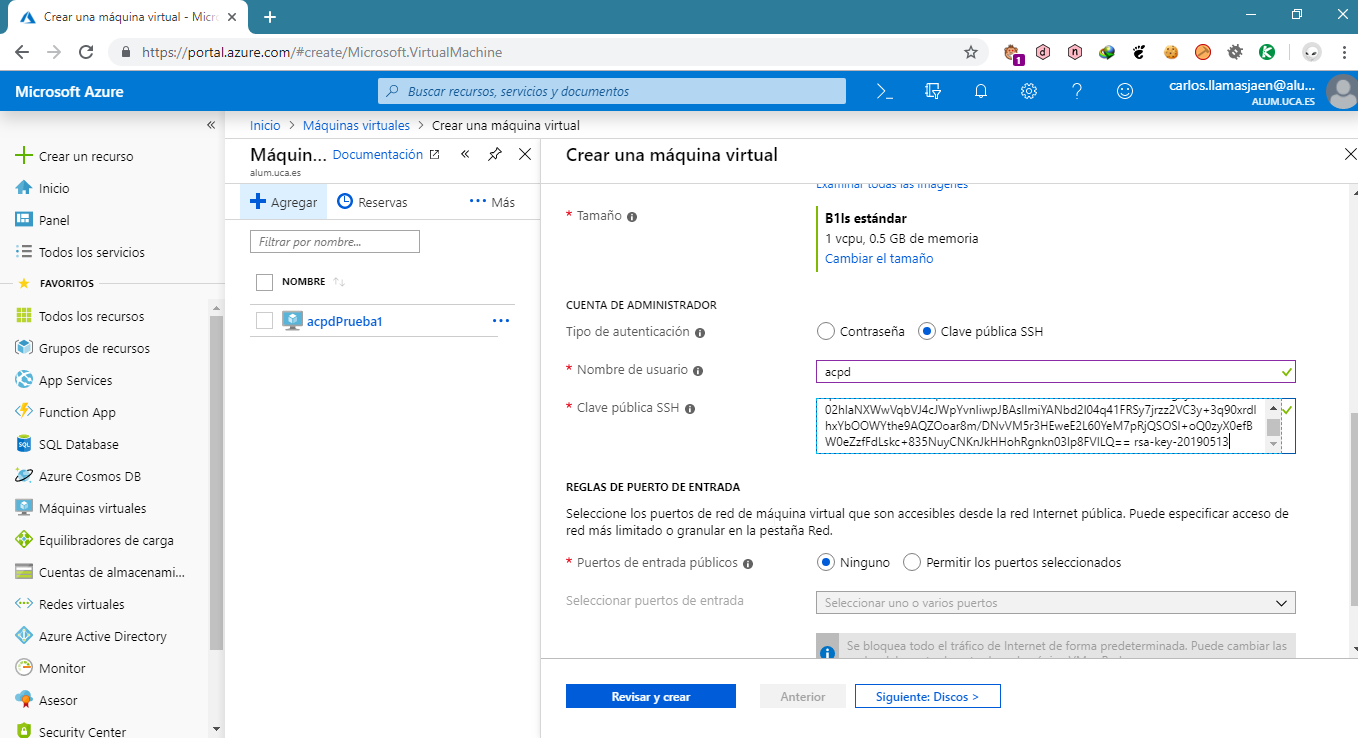
\includegraphics[scale=0.35]{ImagenesAzure/MV/2.png}
		\caption{Establecer autenticación por SSH.}
		\label{Establecer autenticación por SSH}
	\end{figure}
\newpage
	\item Seleccionamos el tamaño de almacenamiento:
	\begin{figure}[h]
		\centering
		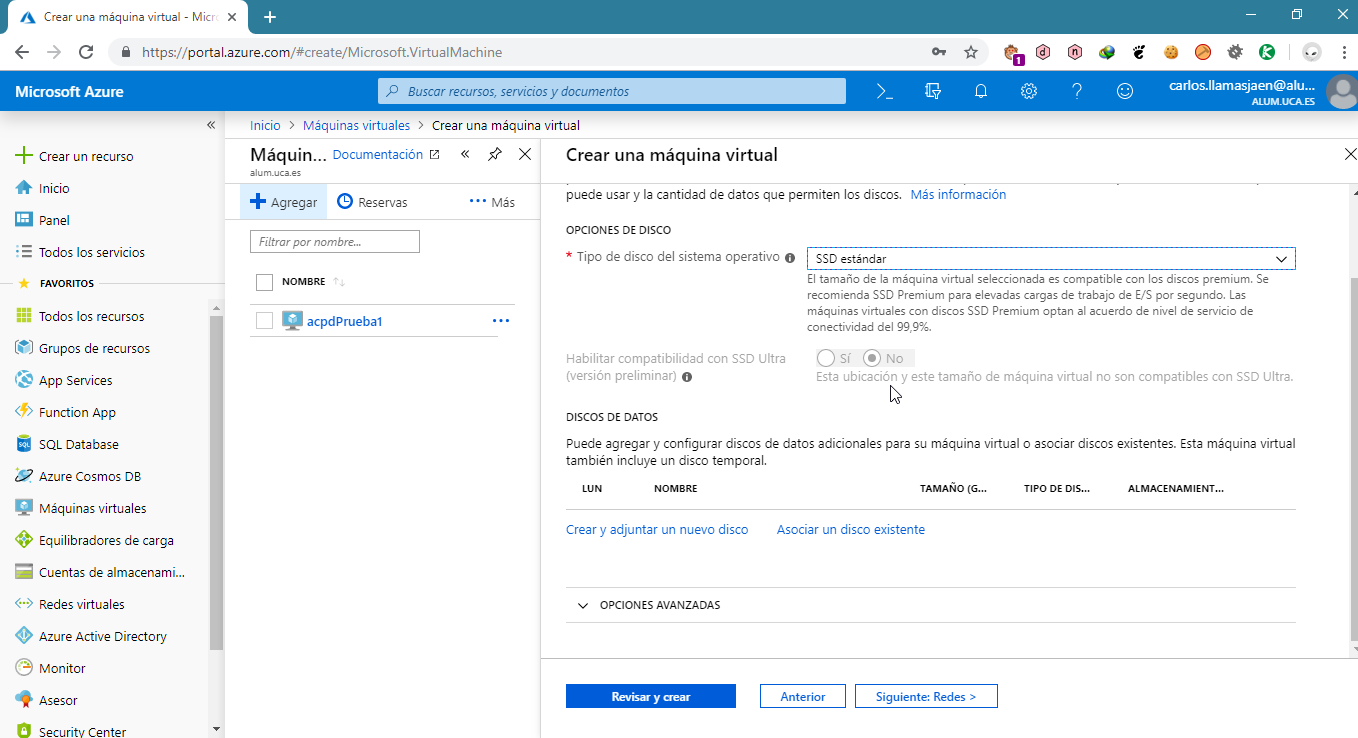
\includegraphics[scale=0.35]{ImagenesAzure/MV/3.png}
		\caption{Selección de almacenamiento.}
		\label{Selección de almacenamiento2}
	\end{figure}
	\item Configuramos las redes virtuales:
	\begin{figure}[h]
		\centering
		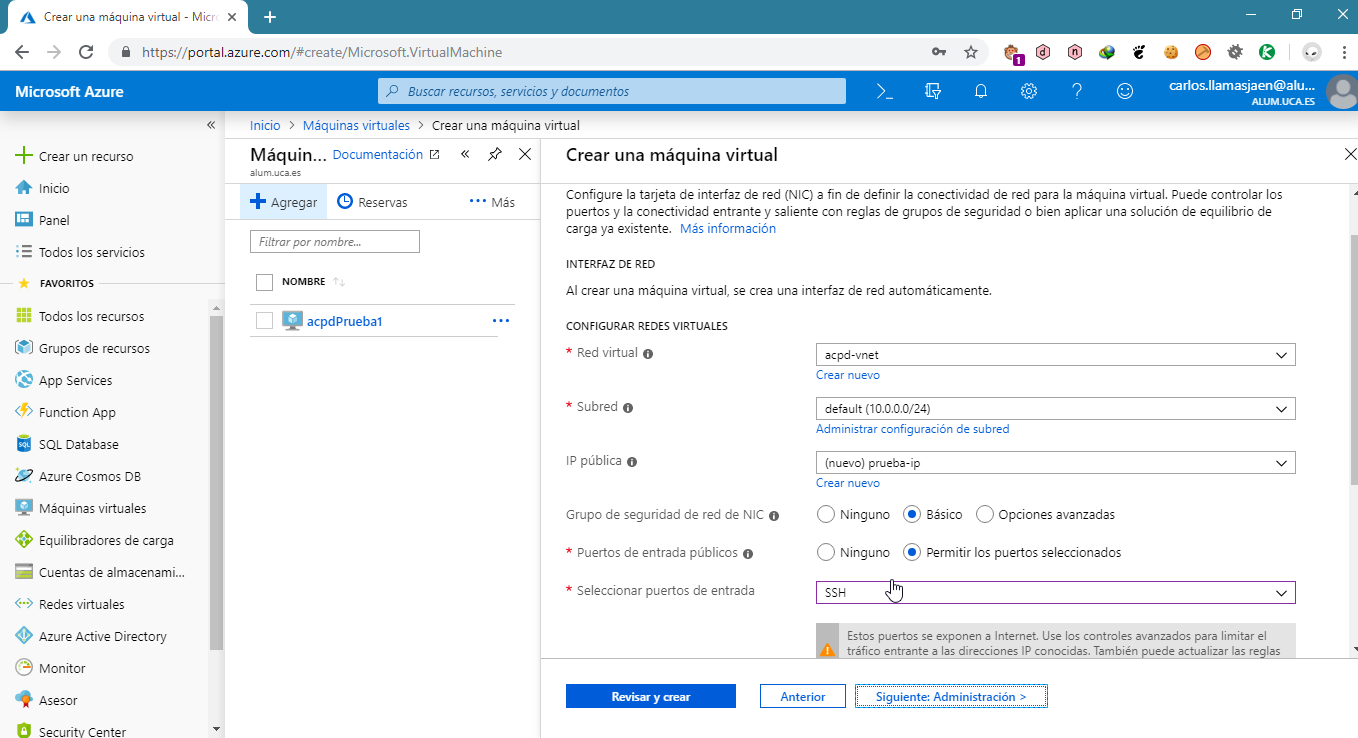
\includegraphics[scale=0.35]{ImagenesAzure/MV/4.png}
		\caption{Configuración de redes virtuales.}
		\label{Configuración de redes virtuales}
	\end{figure}
\newpage
	\item Seleccionamos los puertos de entrada y si queremos equilibrio de carga:
	\begin{figure}[h]
		\centering
		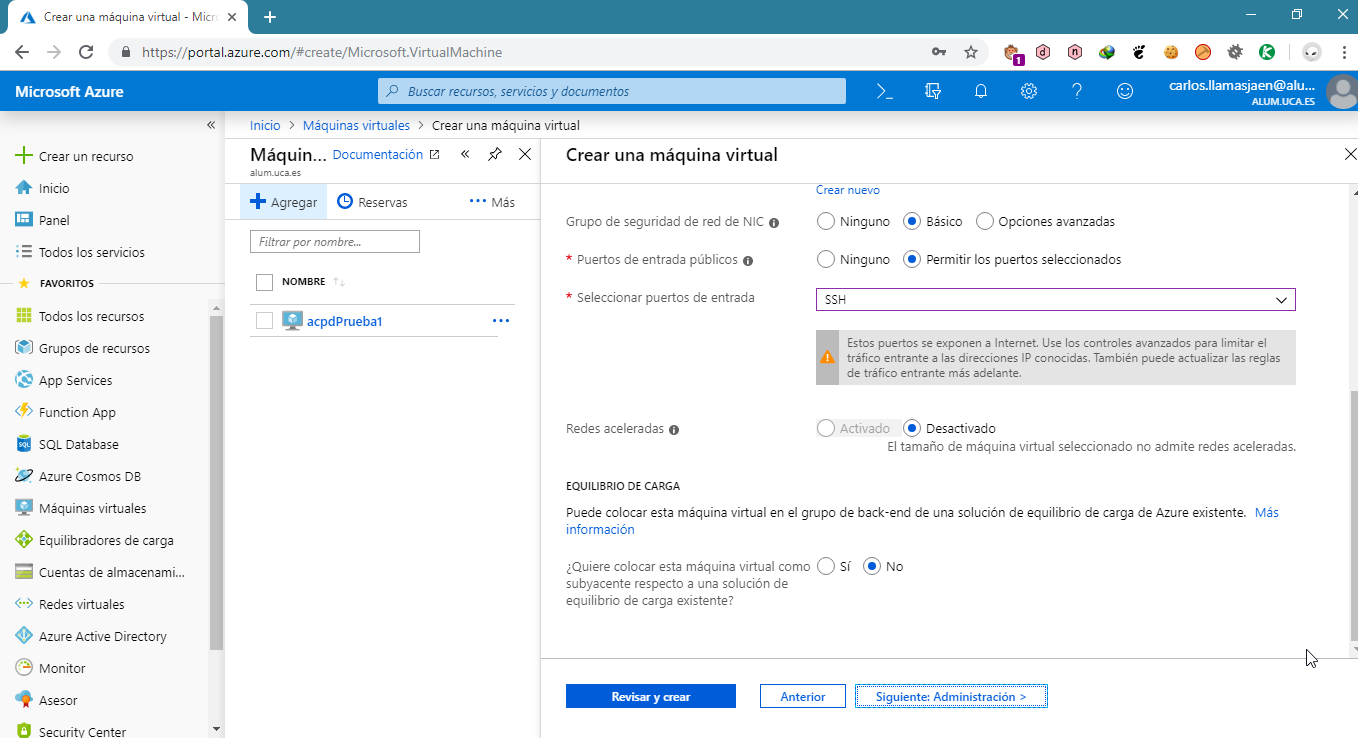
\includegraphics[scale=0.35]{ImagenesAzure/MV/5.png}
		\caption{Selección de entrada y equilibrio de carga.}
		\label{Selección de entrada y equilibrio de carga}
	\end{figure}
	\item Añadimos la configuración de seguridad:
	\begin{figure}[h]
		\centering
		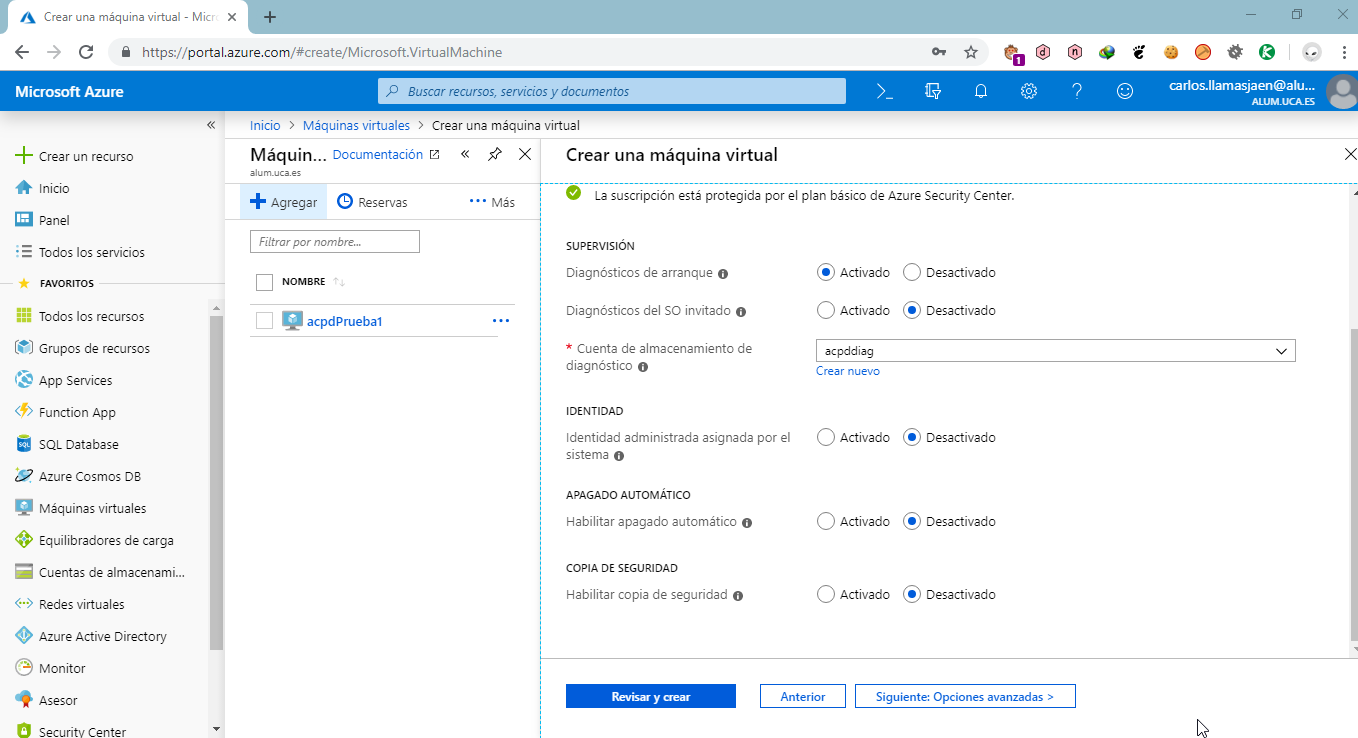
\includegraphics[scale=0.35]{ImagenesAzure/MV/7.png}
		\caption{Configuración de seguridad.}
		\label{Configuración de seguridad}
	\end{figure}
\newpage
	\item Luego veremos las extensiones dentro de las opciones avanzadas:
	\begin{figure}[h]
		\centering
		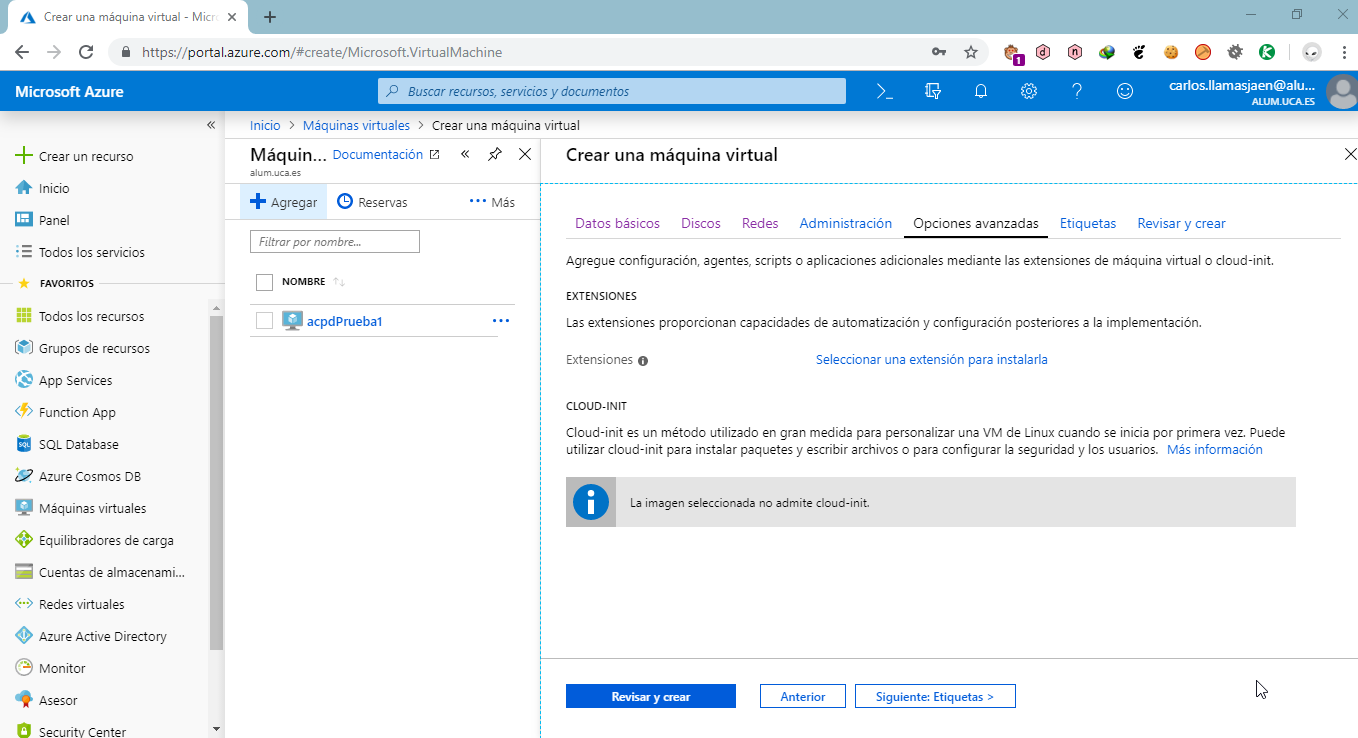
\includegraphics[scale=0.35]{ImagenesAzure/MV/8.png}
		\caption{Opciones avanzadas.}
		\label{Opciones avanzadas}
	\end{figure}
	\item Añadimos las etiquetas que deseemos:
	\begin{figure}[h]
		\centering
		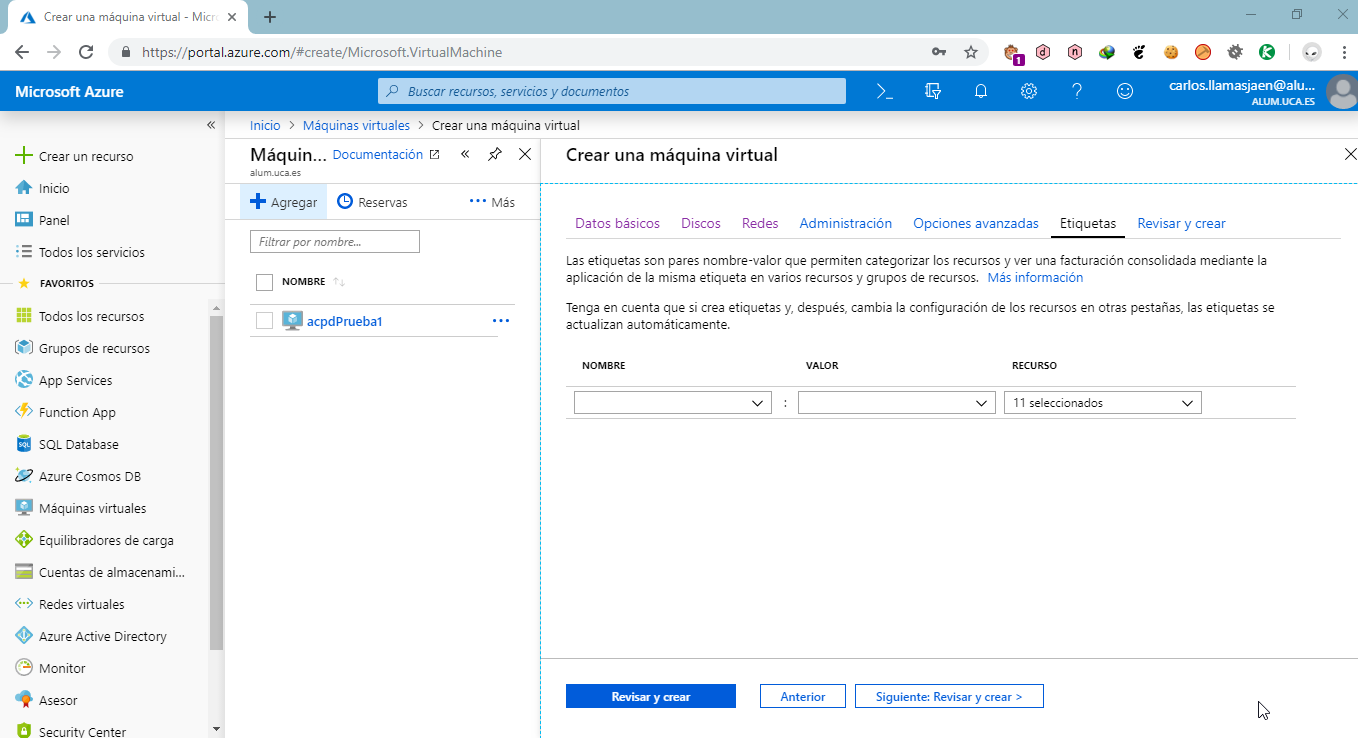
\includegraphics[scale=0.35]{ImagenesAzure/MV/9.png}
		\caption{Añadimos las etiquetas.}
		\label{Añadimos las etiqutas2}
	\end{figure}
\newpage
	\item Finalmente, revisamos la configuración y creamos la máquina virtual:
	\begin{figure}[h]
		\centering
		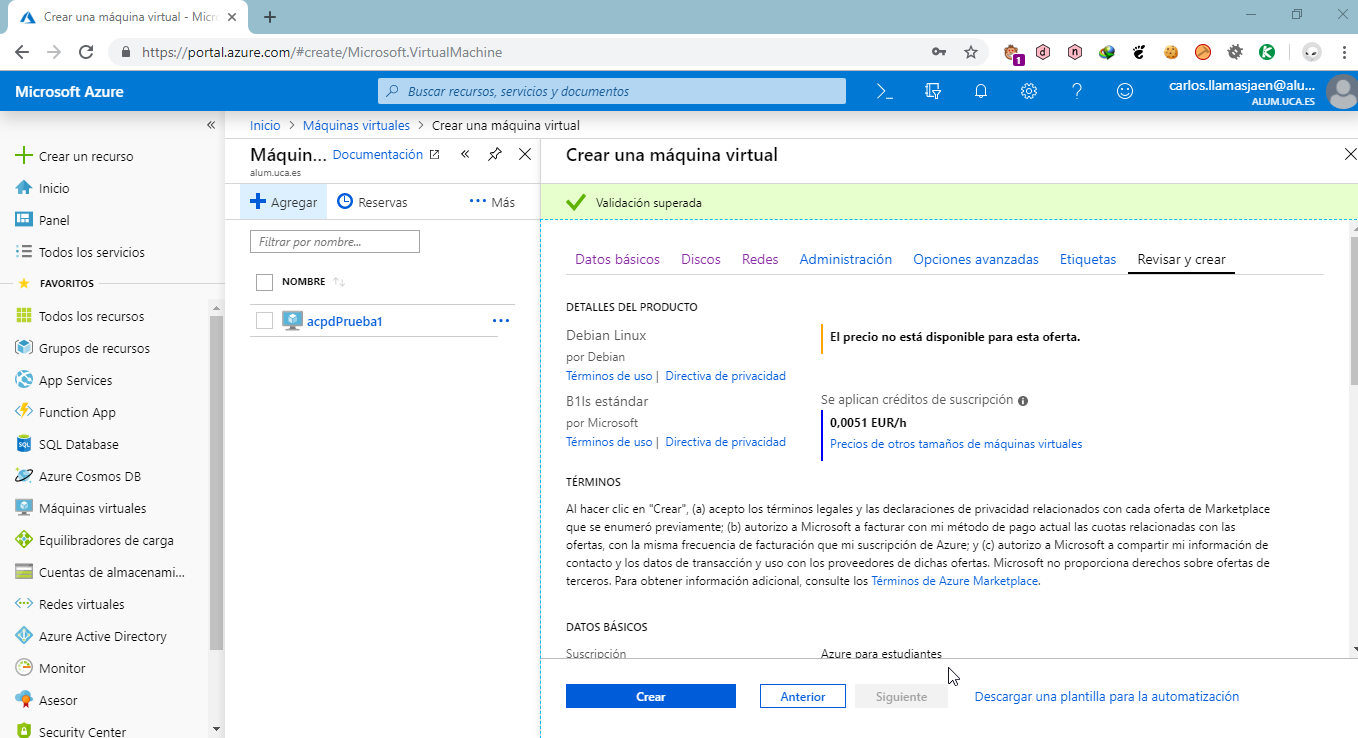
\includegraphics[scale=0.35]{ImagenesAzure/MV/10.png}
		\caption{Revisión de la configuración.}
		\label{Revisión de la configuración}
	\end{figure}
	\item Para conectarnos, lo haremos por ssh a la IP indicada y para ver las especificaciones de la CPU de la máquina virtual usaremos el comando \texttt{cat /proc/cpuinfo}:
	\begin{figure}[h]
		\centering
		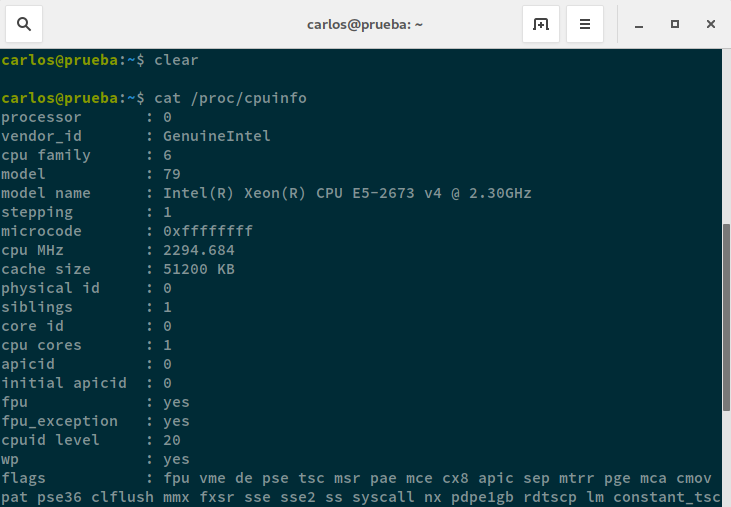
\includegraphics[scale=0.45]{ImagenesAzure/MV/cpuinfo.png}
		\caption{Información del procesador.}
		\label{Información del procesador}
	\end{figure}
\end{enumerate}
	\chapter{Creación de webs en AWS y Azure}
Describir aquí el tipo de máquina virtual que vamos a usar en ambas plataformas y luego, en cada sección, poner los pasos a seguir con sus fotos correspondientes.
\section{Creación de una web en AWS}


\section{Creación de una web en Azure}
	\chapter{Creación de servicios de IoT en AWS y Azure}
Tanto Azure como AWS ofrecen servicios de mensajería entre dispositivos, como por ejemplo colas de mensajes. 

Ambos utilizan MQTT para la comunicación, aunque es posible en Azure utilizar su propio protocolo, pero no ofrece ventaja alguna sobre MQTT.

Vamos a demostrar las características de creación y administración de colas de mensajes y  los dispositivos que se conectan a ella.

Las ventajas de utilizar un servicio para este tipo de proyectos es el ahorro en costes de infraestructura y de seguridad que se tendría que realizar de forma manual, ya que habría que disponer de un servidor dedicado, exponerlo con seguridad a internet. Sin embargo, utilizando estos servicios nos tenemos que preocupar únicamente de desarrollar las aplicaciones, tampoco suponen un coste desorbitado, ya que para pocos dispositivos (50) es gratuito y a partir de ahí, el millón de mensajes entre dispositivos varía entre 0,7 y 1,5 dólares.

Además cabe mencionar la escalabilidad, que es la gran estrella de los servicios en la nube, poder escalar en caso de necesidad sin suponer una gran inversión ni tiempo.

\newpage
\section{Creación de servicios IoT en AWS}
En AWS tenemos que crear primero un Iot Center. AWS es sencillo de conectar, ya que al revés que Azure, en el cuál predomina su propio protocolo, se basa en el protocolo MQTT para transmitir los datos.
\begin{figure}[h]
	\centering
	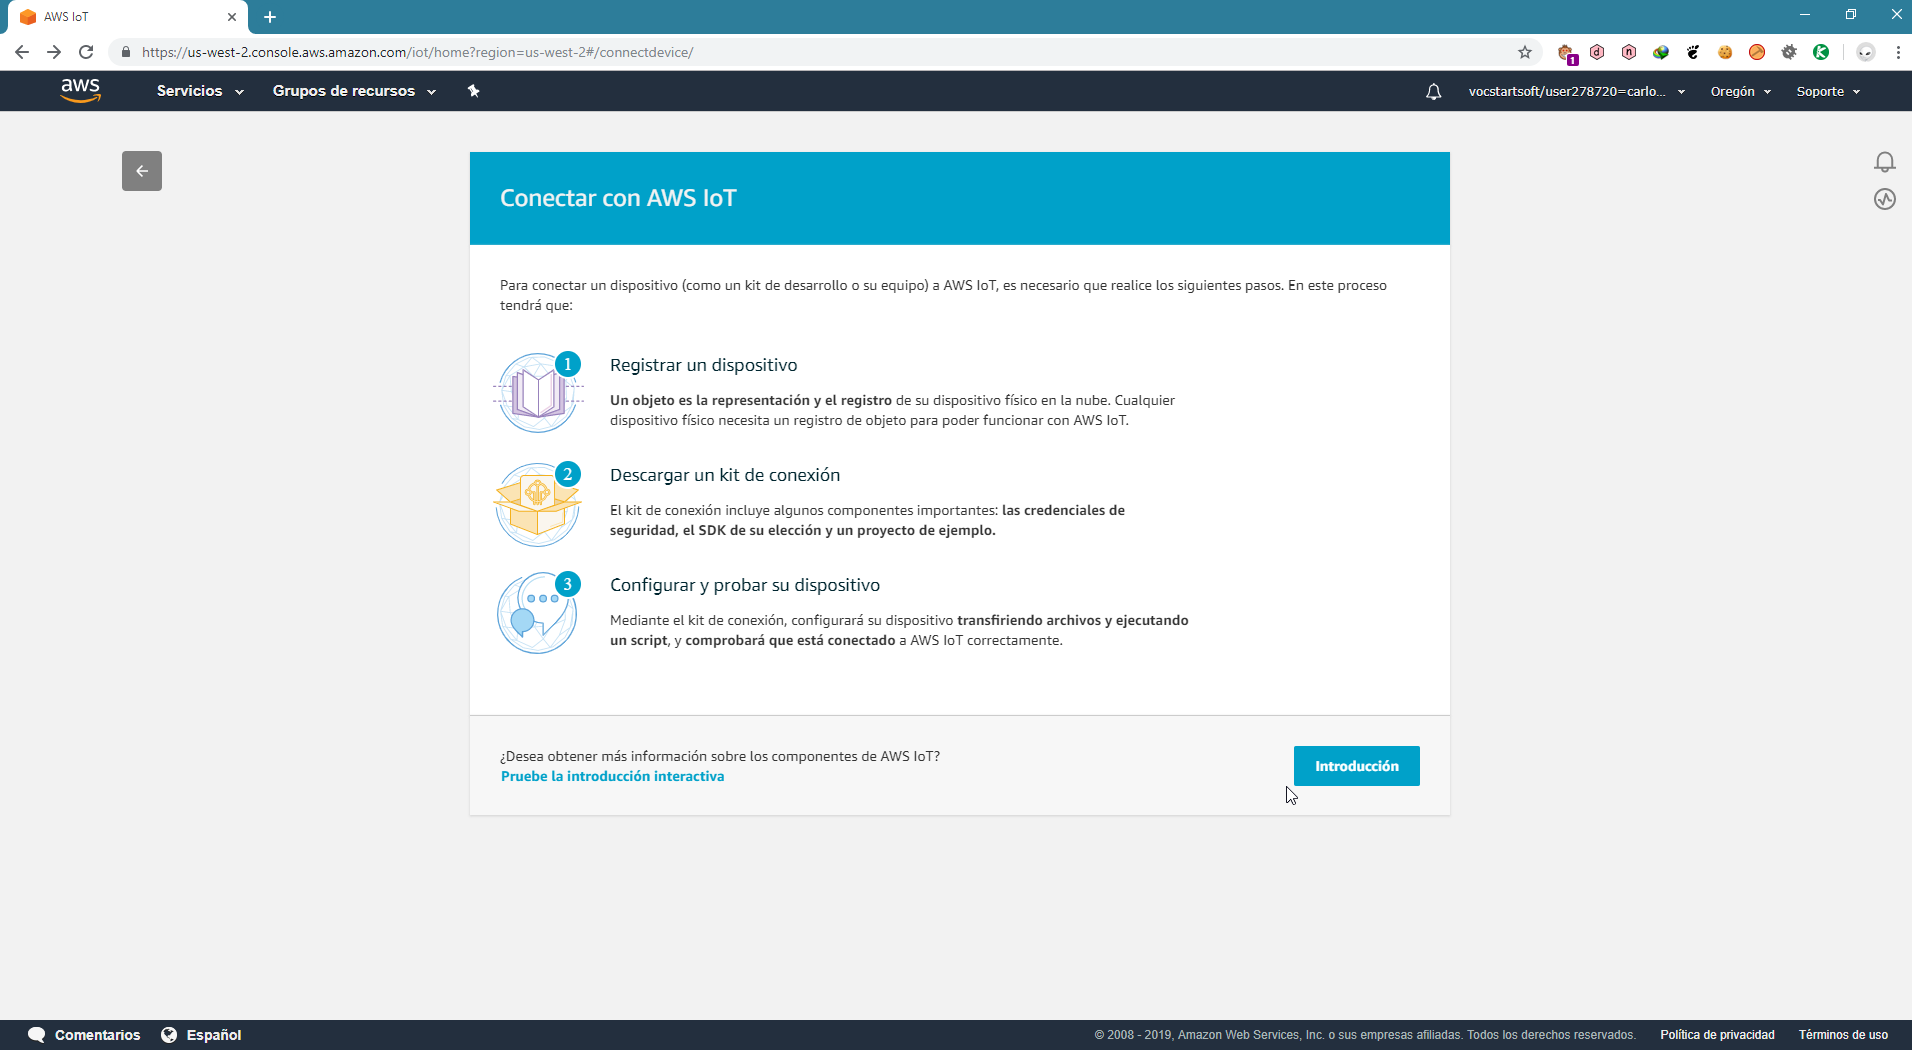
\includegraphics[scale=0.27]{iot_aws/creacion1.png}
	\caption{Creación del centro IOT}
	\label{AWSIOT1}
\end{figure}

Tras ver la introducción, se nos pide seleccionar el lenguaje a utilizar y el sistema operativo, para así poder descargar las herramientas que nos permitirán empezar a hablarnos con AWS a una cola MQTT.

\begin{figure}[h]
	\centering
	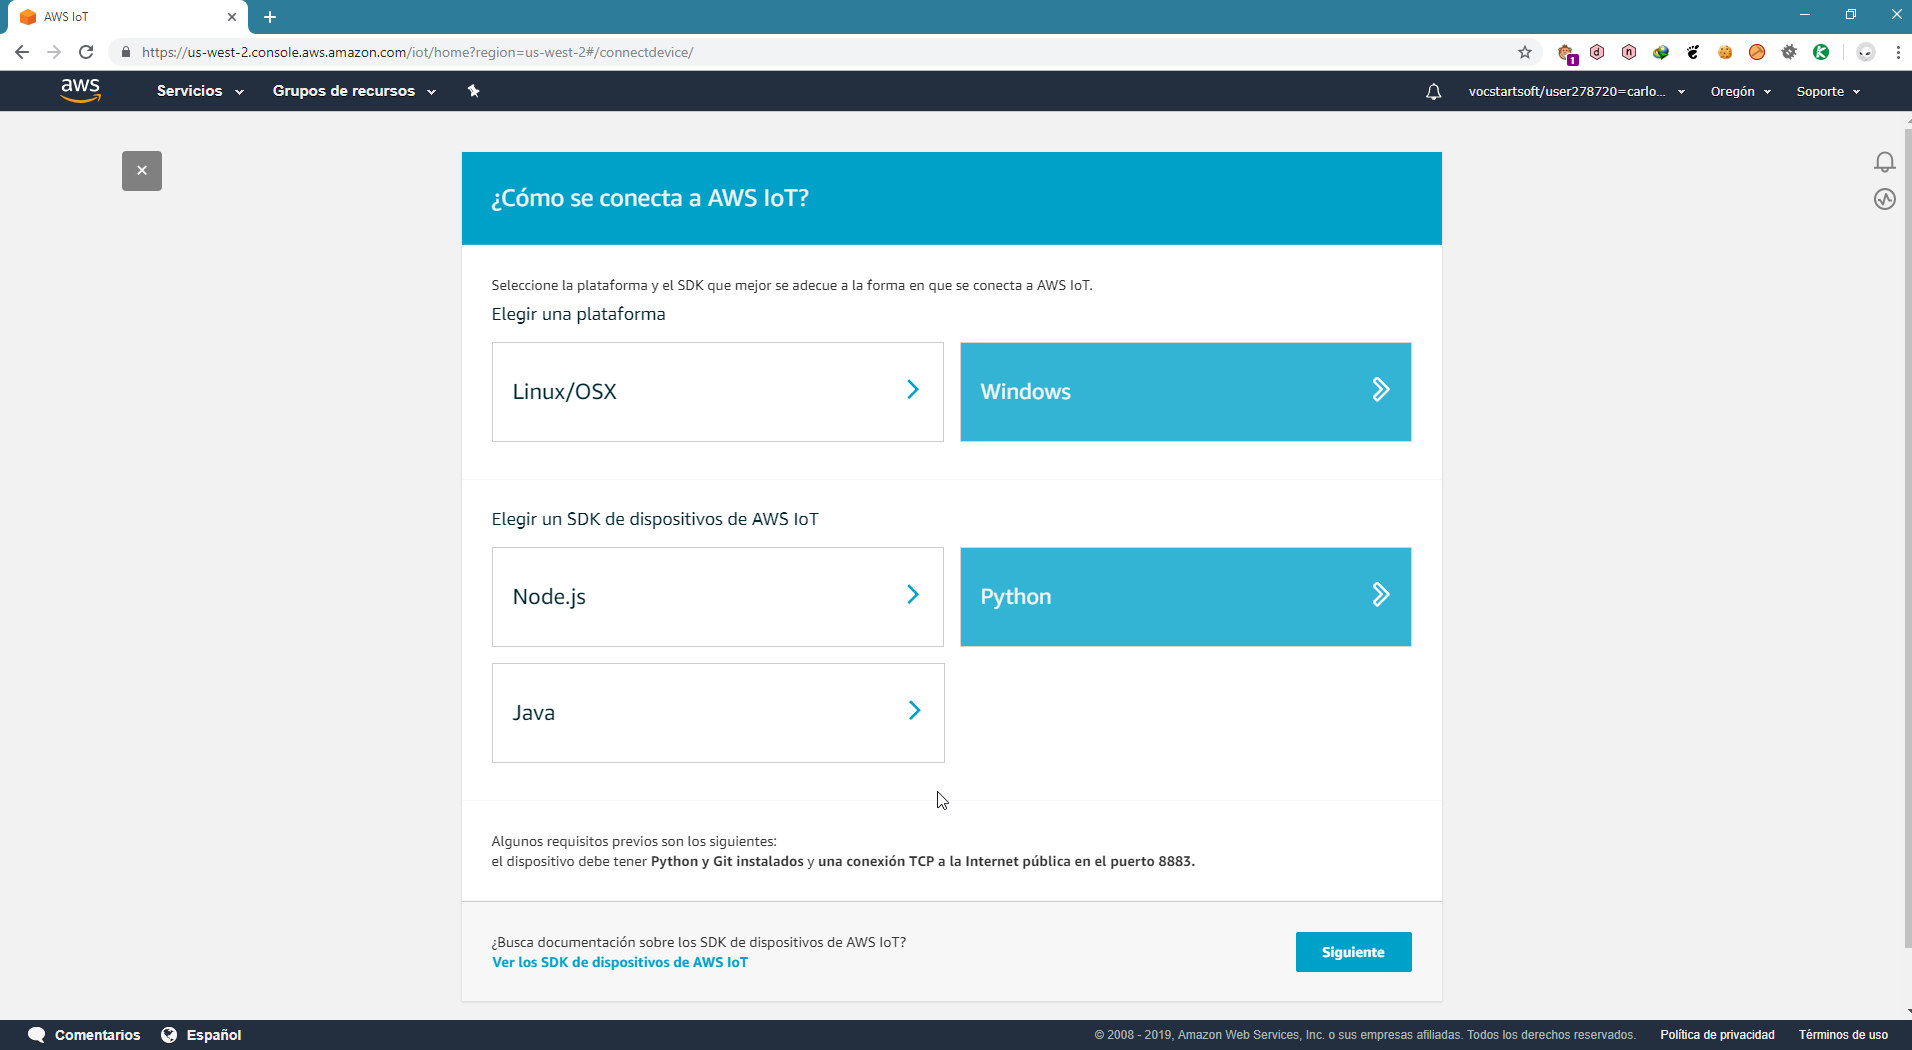
\includegraphics[scale=0.27]{iot_aws/creacion2.png}
	\caption{Selección del sistema operativo}
	\label{AWSIOT2}
\end{figure}

\newpage
Posteriormente tenemos que asignarle un nombre al objeto / dispositivo para poder reconocerlo en las métricas, ya que la autentificación, como se verá más adelante se realiza por medio de certificados.

\begin{figure}[h]
	\centering
	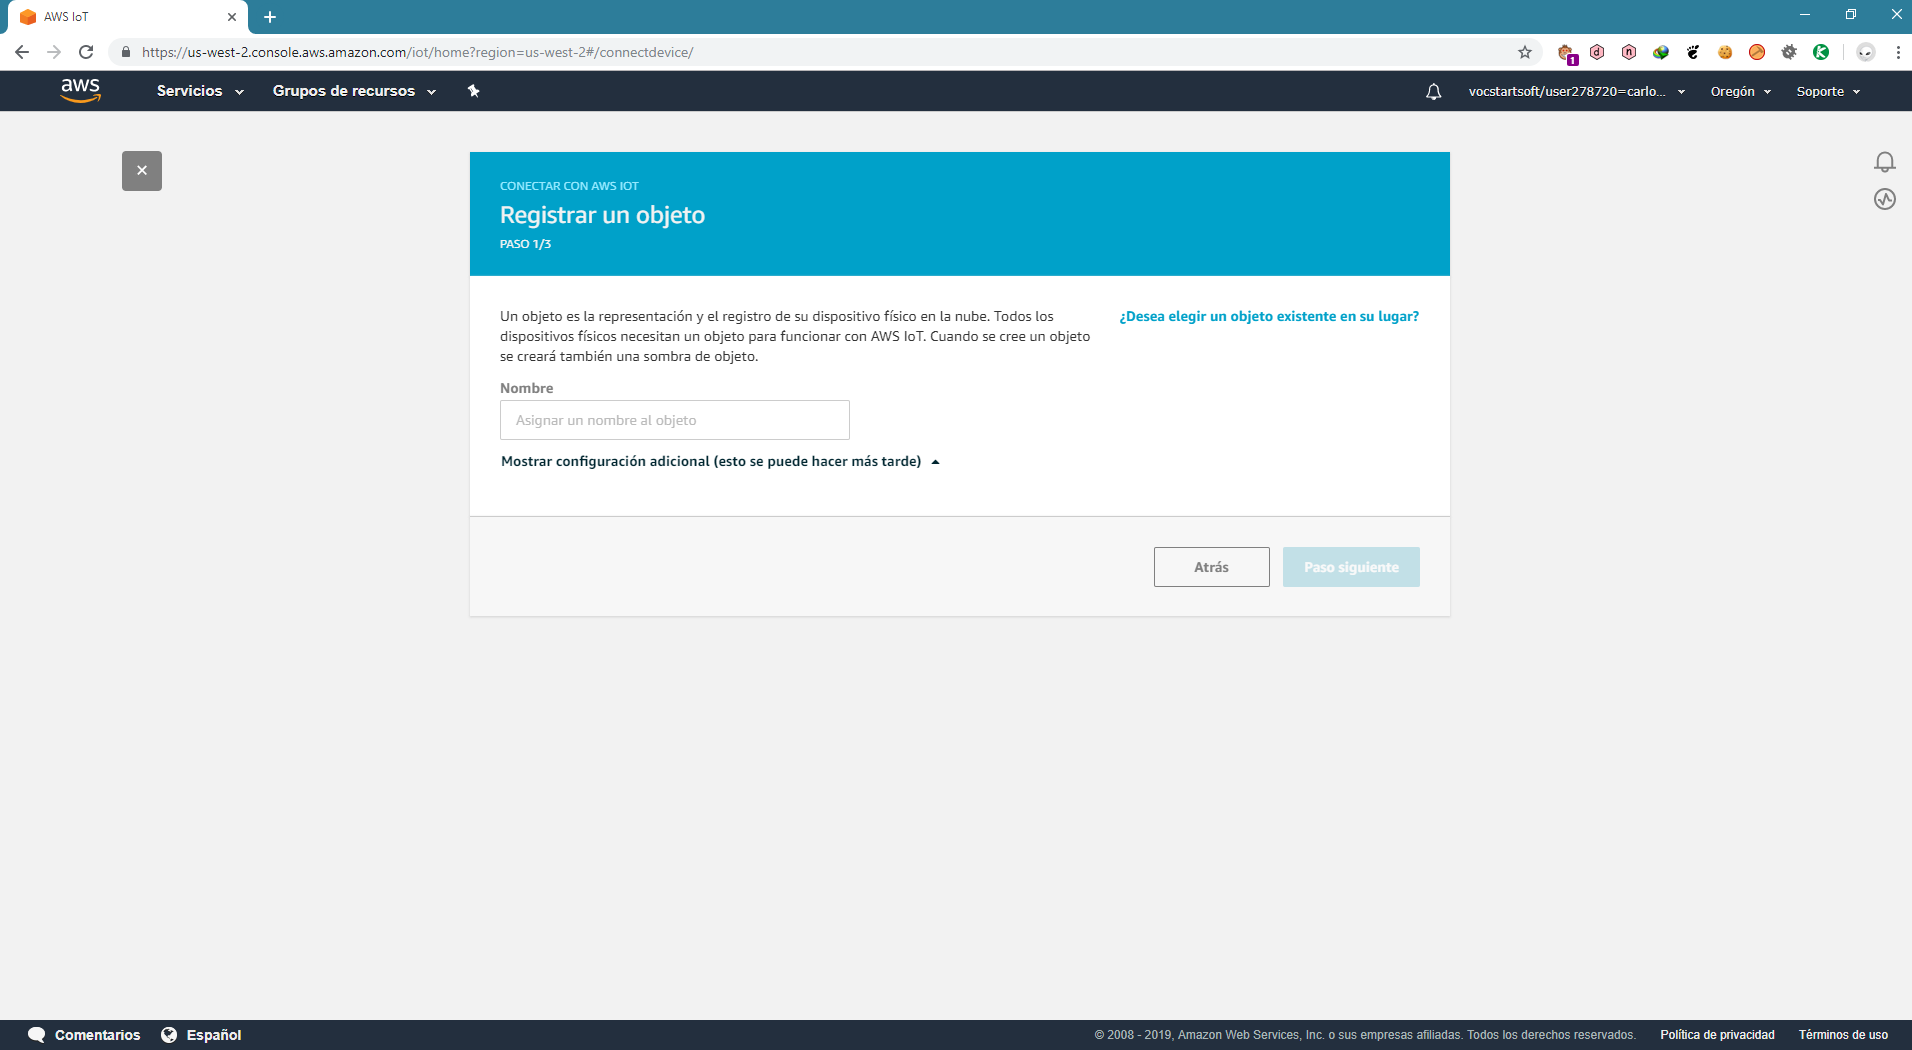
\includegraphics[scale=0.27]{iot_aws/creacion3.png}
	\caption{Selección del nombre del dispositivo}
	\label{AWSIOT3}
\end{figure}

Una vez creado el nombre, estamos listos para ejecutar los ejemplos que vienen con el kit de desarrollo, viene con todo lo necesario para empezar a comunicarnos con AWS, tanto los ejemplos como los certificados necesarios para autentificar el objeto anterior.

\begin{figure}[h]
	\centering
	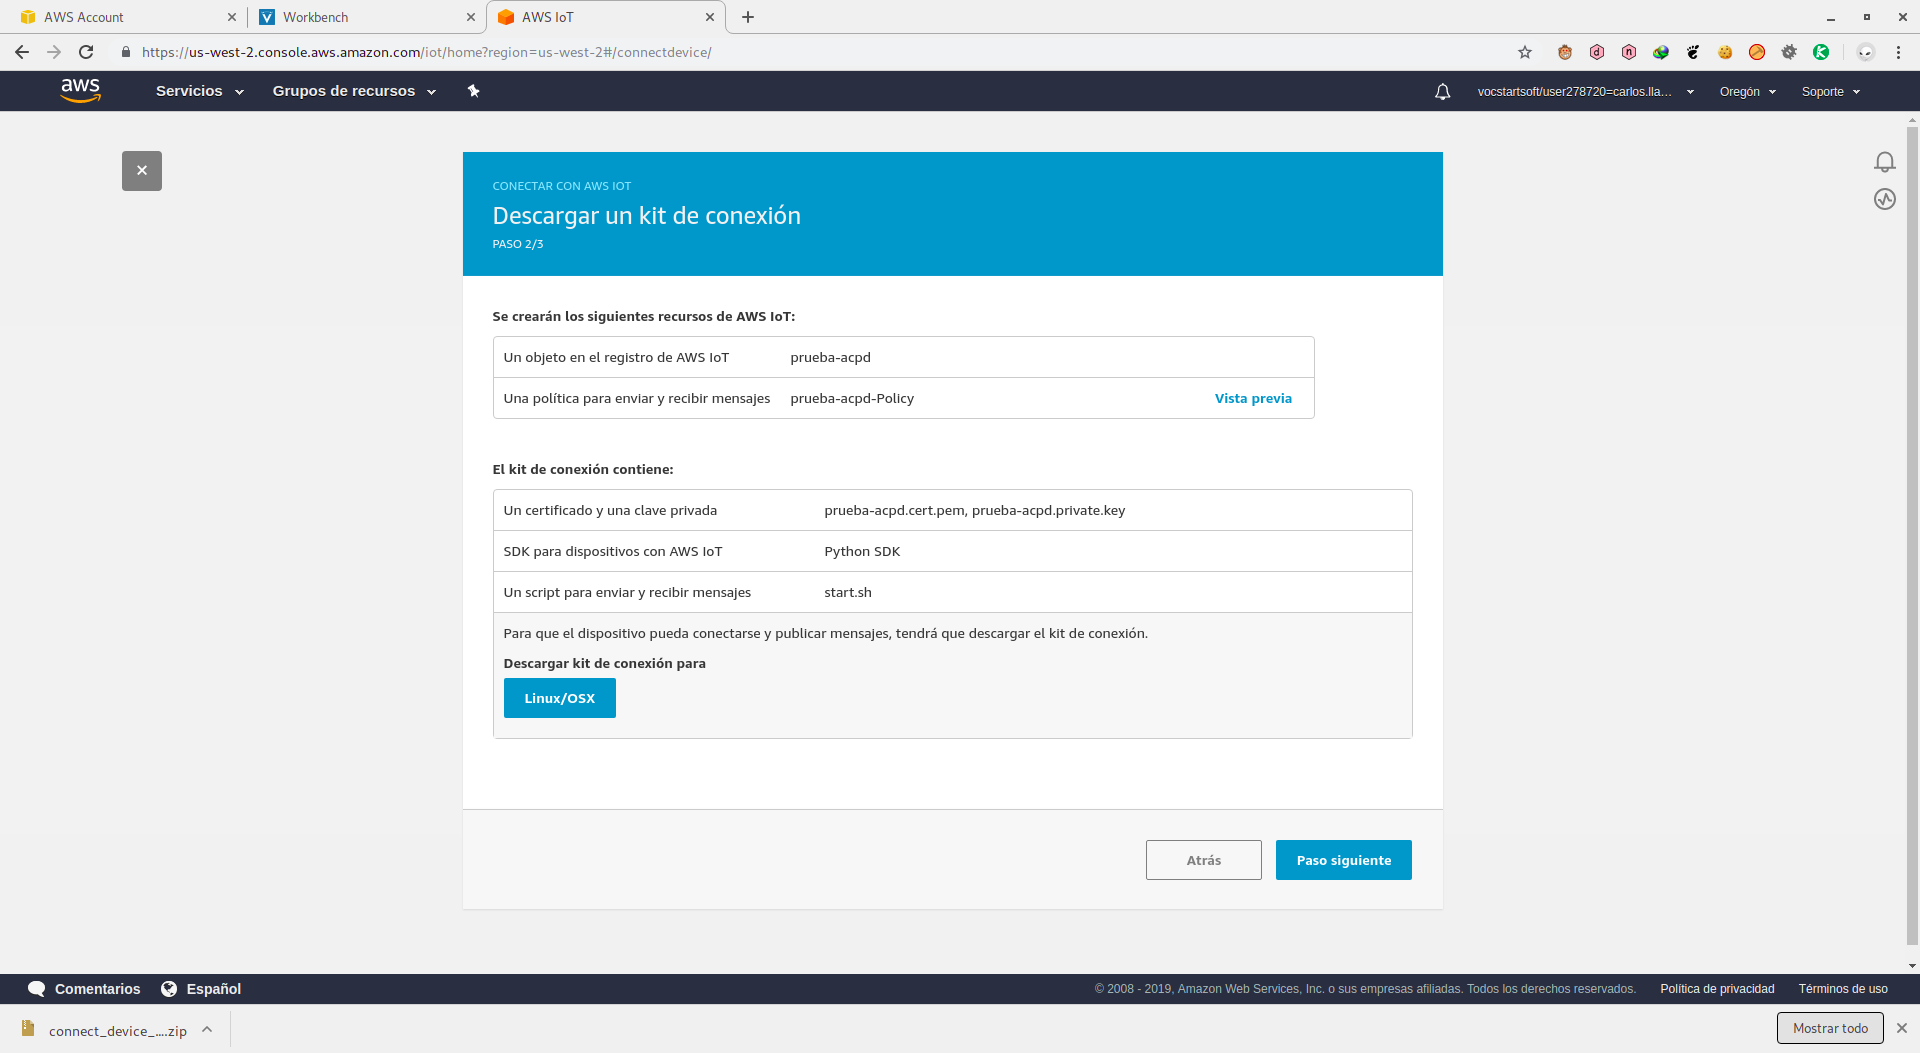
\includegraphics[scale=0.2]{iot_aws/creacion4.png}
	\caption{Descarga del kit de prueba}
	\label{AWSIOT4}
\end{figure}

\newpage
Posteriormente lo ejecutamos y empezaremos a ver como llegan mensajes y la aplicación de Amazon es capaz de leerla.

\begin{figure}[h]
	\centering
	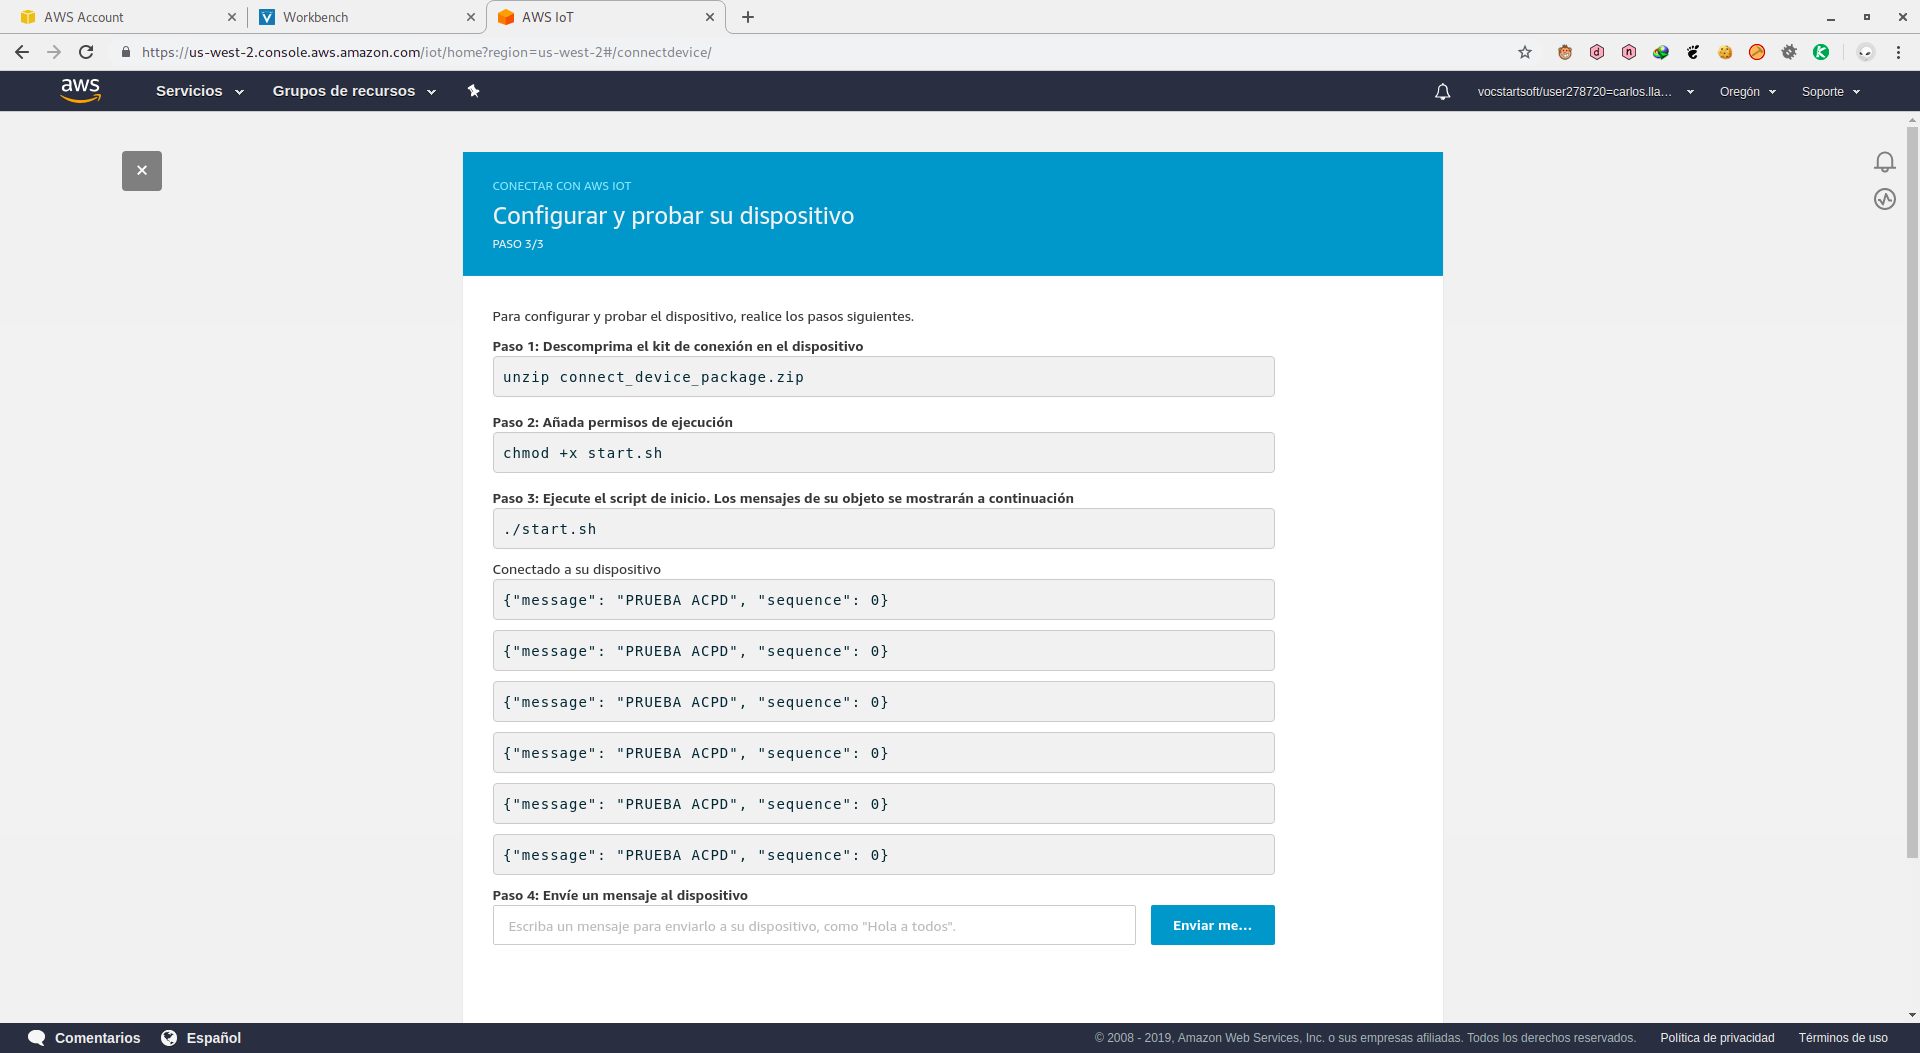
\includegraphics[scale=0.2]{iot_aws/creacion5.png}
	\caption{Prueba de ejecución}
	\label{AWSIOT5}
\end{figure}

Una vez llegado a este paso tenemos listo todo lo necesario para empezar a desarrollar nuestras aplicaciones sobre IoT.

También resulta interesante, añadir nuevos dispositivos / objetos, visualizar métricas de mensajes, modificar las políticas de seguridad de los dispositivos.

Para ello disponemos en el centro de IoT la sección de métricas:

\begin{figure}[h]
	\centering
	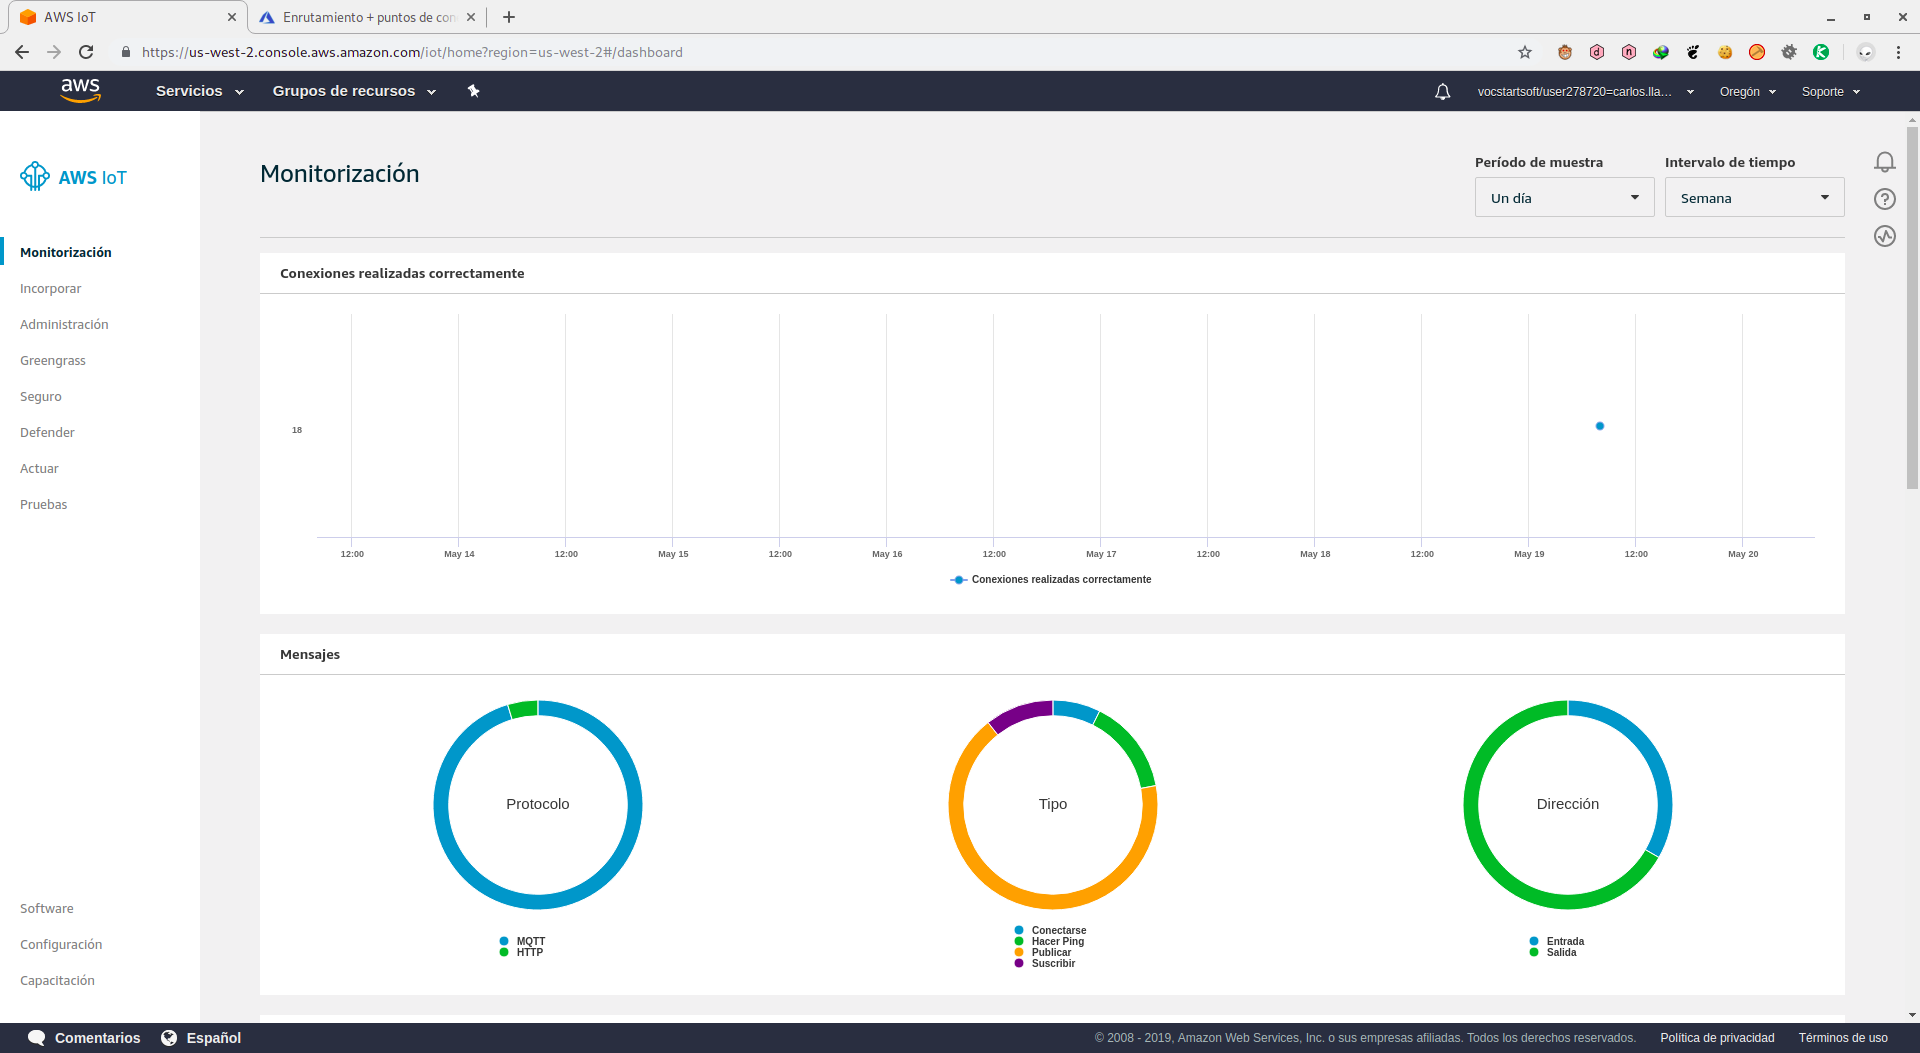
\includegraphics[scale=0.2]{iot_aws/centro.png}
	\caption{Visualización de las métricas}
	\label{AWSIOT6}
\end{figure}

\newpage
También disponemos una interfaz de gestión de dispositivos, donde podemos gestionar los parámetros de estos dispositivos:


\begin{figure}[h]
	\centering
	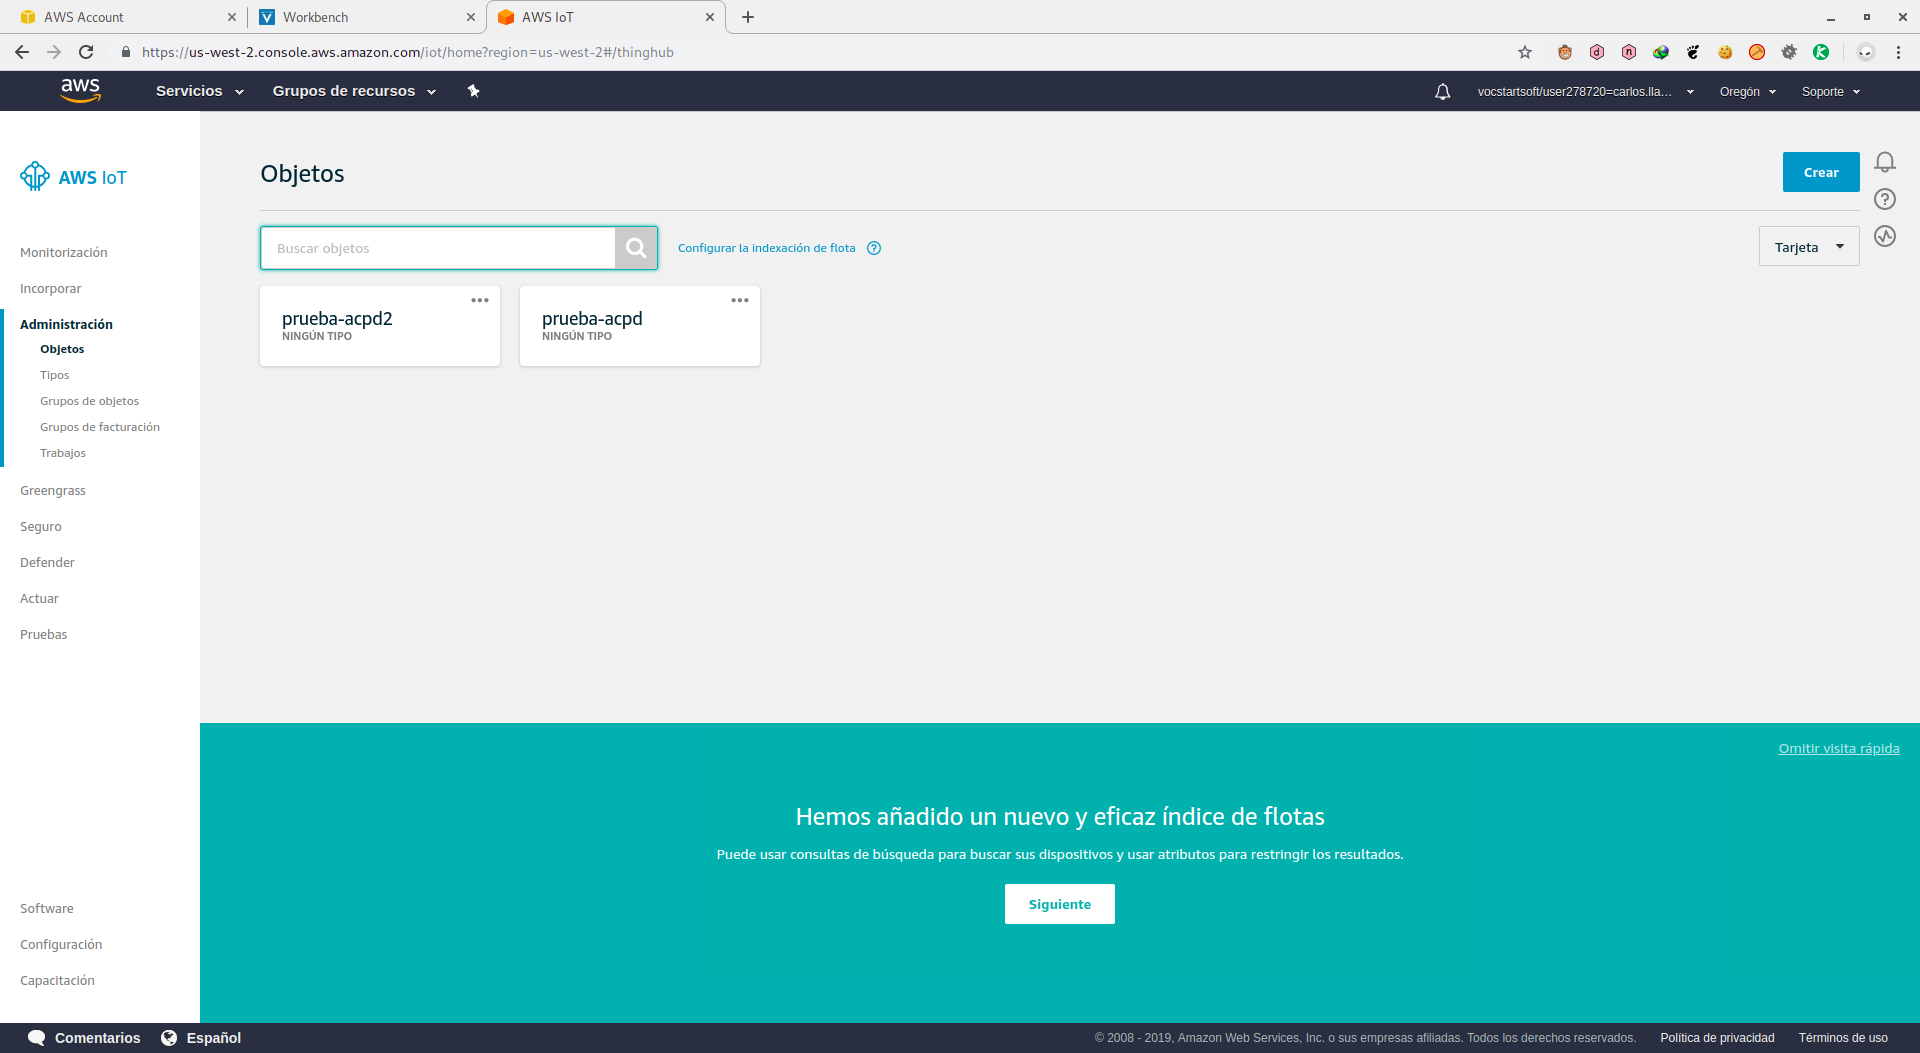
\includegraphics[scale=0.2]{iot_aws/dispositivos.png}
	\caption{Visualización del número de dispositivos}
	\label{AWSIOT7}
\end{figure}

\begin{figure}[h]
	\centering
	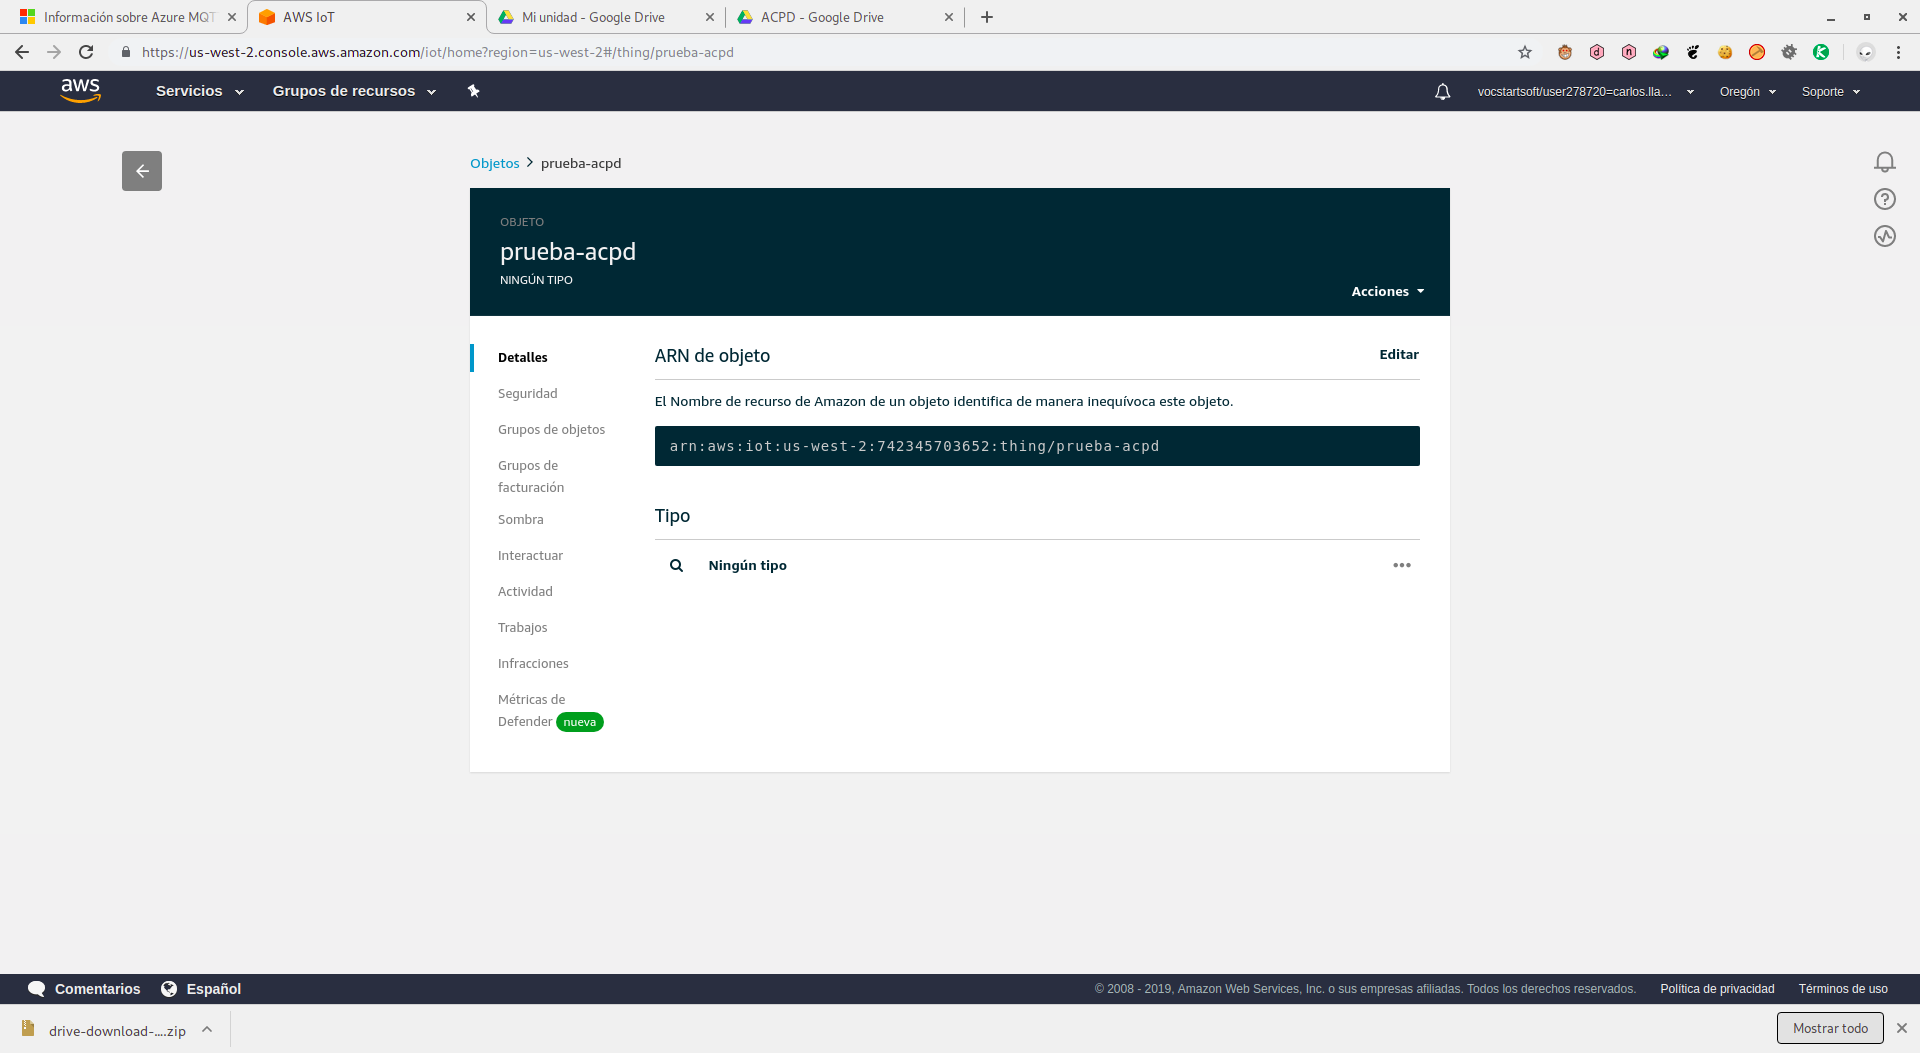
\includegraphics[scale=0.2]{iot_aws/dispositivos2.png}
	\caption{Gestión de un dispositivo}
	\label{AWSIOT8}
\end{figure}

\section{Creación de servicios IoT en Azure}
Ahora vamos a centrarnos en el servicio de Microsoft, la ventaja que tiene sobre AWS es la multiplataforma y la dedicación de Microsoft al IoT, ya que tiene distintas versiones de Windows adaptadas al IoT. Mientras que AWS soporta únicamente Java, Node.JS y Python, Azure lo expande con su plataforma estrella, .NET Core, a la que le está dando un gran empujón en los últimos años.

La ventaja de poder usar .NET Framework o .NET Core para desarrollar estas aplicaciones es la integración con el IDE Visual Studio, ya que prácticamente con 1 click podemos enviar la aplicación en la nube, como se vió en el apartado de desarrollo de servicios web.

Lo primero que hay que realizar en Azure es dar de alta un Centro de IoT o IoT Hub. Los grupos de recursos de Azure van enfocados a agrupar los recursos de cara a la facturación, en este caso al disponer de crédito gratuito podemos ignorarlo, con cuidado de no sobrepasar los límites.

\begin{figure}[h]
	\centering
	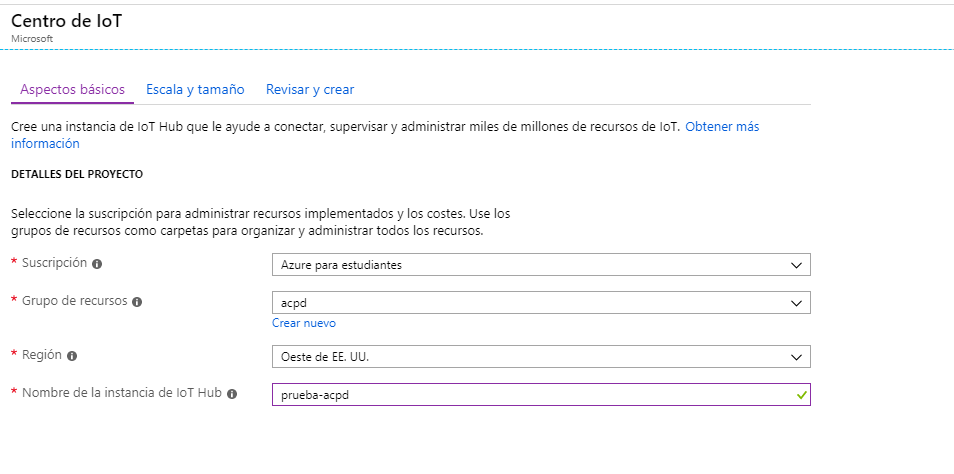
\includegraphics[scale=0.5]{iot_azure/primera.png}
	\caption{Creación de un centro IoT}
	\label{AZIOT1}
\end{figure}

Lo siguiente que se nos pide es la escala, a diferencia de AWS que no necesita escalar, si no que cobra por tramos de mensajes, Azure es necesario predefinir una escala, aunque no lleguemos a ella siempre se nos cobrará lo mismo. En este caso Azure tiene una versión gratuita para 8000 mensajes diarios.

\begin{figure}[h]
	\centering
	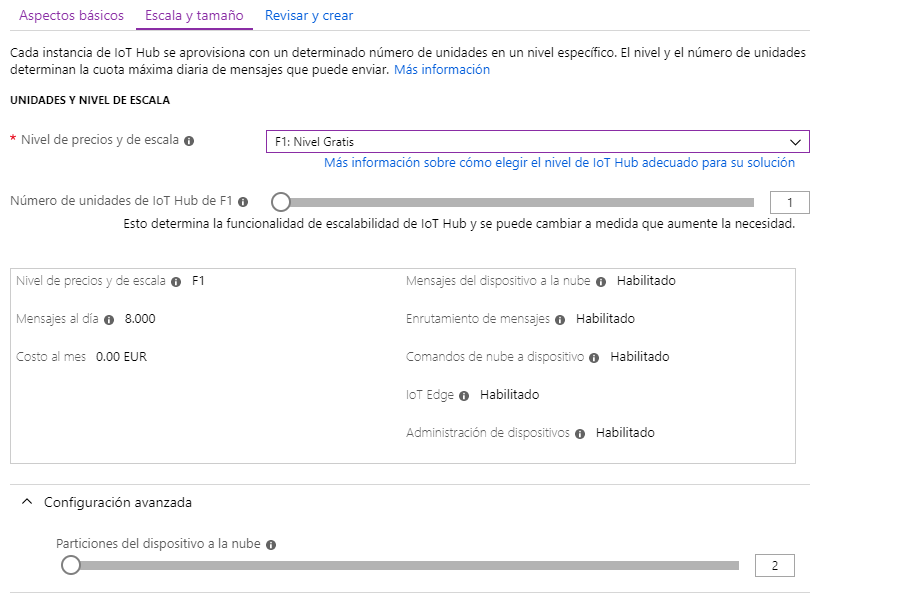
\includegraphics[scale=0.5]{iot_azure/escala.png}
	\caption{Selección de la escala}
	\label{AZIOT2}
\end{figure}

\newpage
Lo próximo que hay que realizar es añadir un dispositivo nuevo. A diferencia de AWS, Azure sí que te deja poner una clave en vez que utilizar certificados.

\begin{figure}[h]
	\centering
	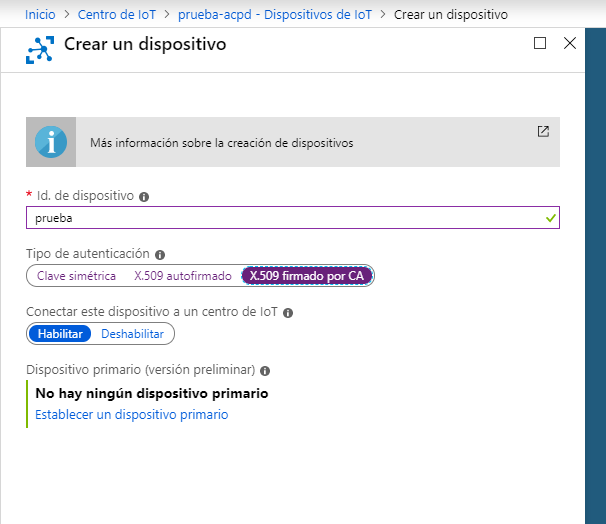
\includegraphics[scale=0.5]{iot_azure/dispositivo.png}
	\caption{Creación de dispositivo}
	\label{AZIOT3}
\end{figure}

Podemos ver los dispositivos en la lista de dispositivos.


\begin{figure}[h]
	\centering
	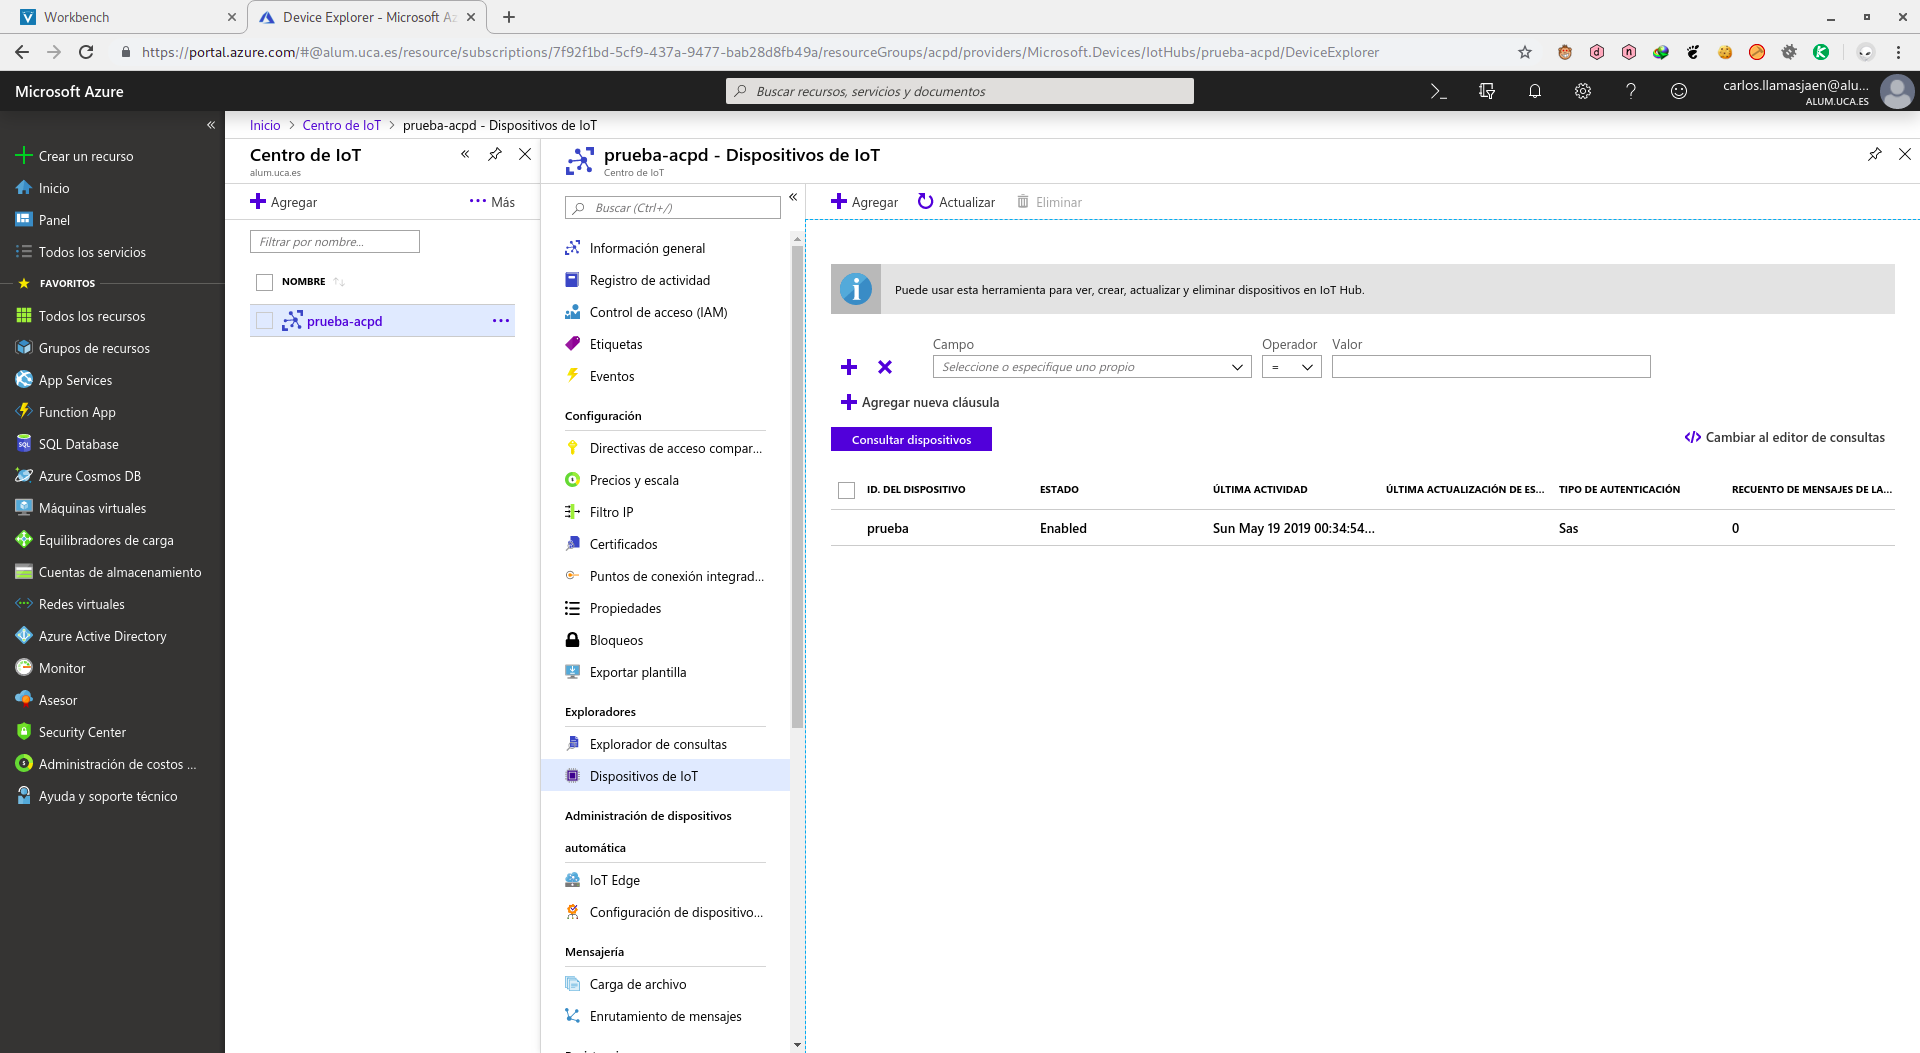
\includegraphics[scale=0.2]{iot_azure/dispositivos.png}
	\caption{Lista de dispositivo}
	\label{AZIOT4}
\end{figure}

\newpage
Una vez listo podemos volver al centro de IOT. Desde aquí podemos establecer políticas de seguridad, filtros, gestionar certificados, mirar métricas, eventos y gestionar la mensajería.

\begin{figure}[h]
	\centering
	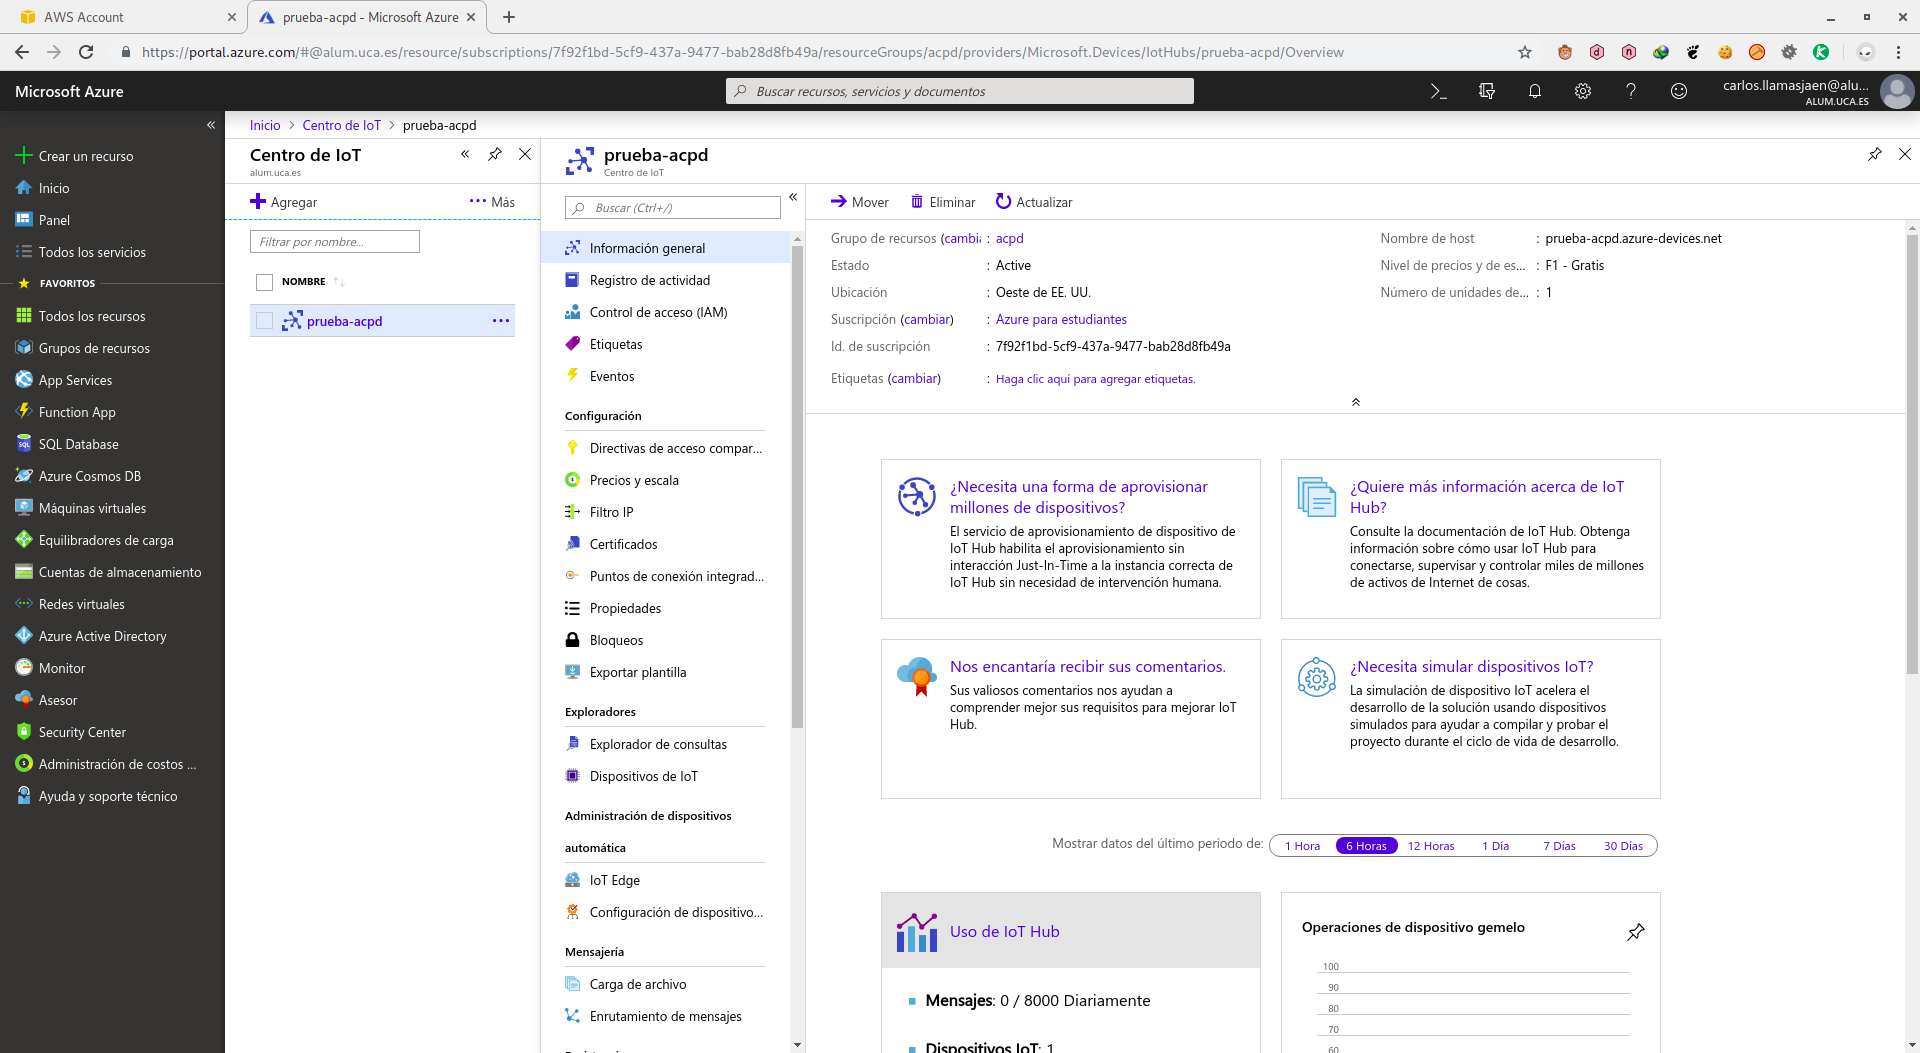
\includegraphics[scale=0.2]{iot_azure/centro.png}
	\caption{Centro de IoT}
	\label{AZIOT5}
\end{figure}

Pues con todo esto listo vamos a probar a ejecutar un ejemplo, para ello tenemos que crear otro dispositivo más y obtener las claves, es posible que haya que utilizar la CLI de Azure, que es de pago, ya que tiene que crear una pequeña cuenta de almacenamiento para poderla usar.


\begin{figure}[h]
	\centering
	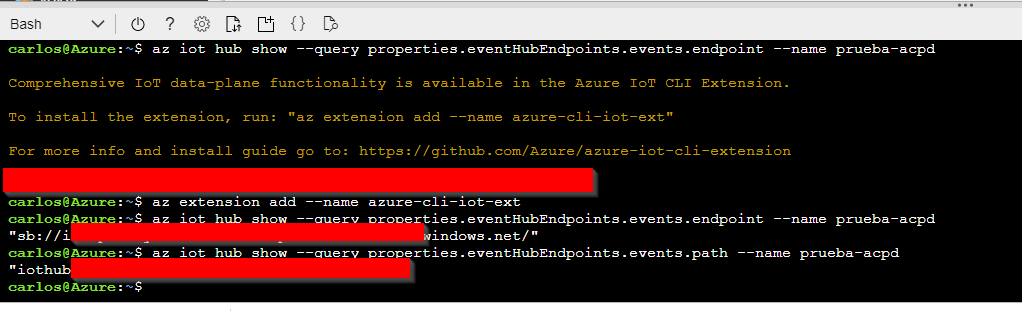
\includegraphics[scale=0.6]{iot_azure/azure_cli.png}
	\caption{Utilización de la Azure CLI para obtener las claves de los dispositivos.}
	\label{AZIOT6}
\end{figure}

\newpage

Una vez establecidas las claves, probamos un ejemplo que hay de IoT Hub, este ejemplo un publicador envía la temperatura de una sala y un suscriptor la recibe. En rojo aparece marcados los mensajes correspondientes que se envían desde el publicador y aparece en el suscriptor.

\begin{figure}[h]
	\centering
	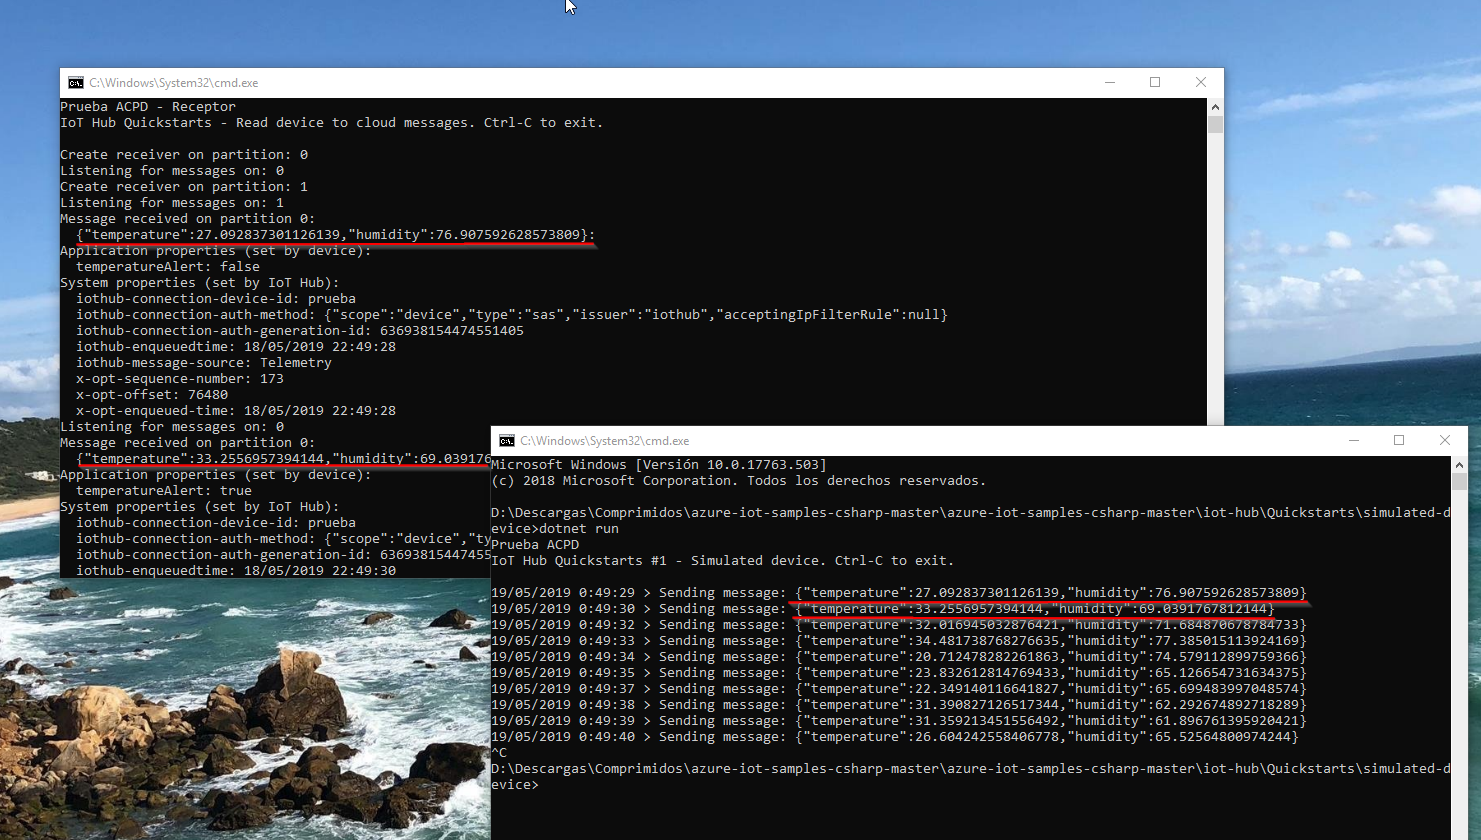
\includegraphics[scale=0.4]{iot_azure/mensajes.png}
	\caption{Ejemplo de IoT}
	\label{AZIOT7}
\end{figure}


	
	\part{Anexo}
	\chapter{Referencias}
En este capítulo se detallarán las referencias consultadas a la hora de redactar este documento.
\begin{itemize}
	\item Documentación oficial de AWS: \url{https://aws.amazon.com/es/}.
	\item Documentación oficial de Azure: \url{https://azure.microsoft.com/es-es/}.
	\item \url{https://es.wikipedia.org/wiki/Amazon_Web_Services}.
	\item \url{https://es.wikipedia.org/wiki/Middleware}.
	\item \url{https://revistadigital.inesem.es/informatica-y-tics/cloud-computing-con-amazon/}.
	\item \url{https://docs.aws.amazon.com/es_es/general/latest/gr/aws_service_limits.html}.
	\item \url{https://azure.microsoft.com/es-es/free/free-account-students-faq/}.
\end{itemize}
	
\end{document}
